% Document Created June 23, 1993 on B2 C2
% AMS-Tex document
% Author Thomas C. Hales
% Reformatted March 2015

\documentclass{amsart}

%Packages
\usepackage{graphicx}
\usepackage{amsfonts}
\usepackage{enumitem}
\usepackage{amscd}
\usepackage{amssymb}
\usepackage{alltt}
\usepackage{txfonts}
%tikz graphics
%\usepackage{xcolor} % to remove color.
\usepackage{tikz} 
\usetikzlibrary{chains,shapes,arrows,shadings,trees,matrix,%
  positioning,intersections,decorations,%
  decorations.markings,decorations.pathmorphing,backgrounds,%
  fit,calc,fadings,decorations.pathreplacing}



%\magnification=\magstep1
%\parindent=0pt
%\baselineskip=1.5\baselineskip
%\parskip=.66\baselineskip
%\pretolerance=10000  % turn off hyphenation
%\raggedbottom        % 

%\UseAMSsymbols
%\loadmsbm
%\loadeufm
\font\headfont=cmcsc10 scaled\magstep1

% \def\star{\hbox to 0pt{\hskip -10pt $\bullet$ \hss}}  %compare Knuth, Exercise 14.28
% \def\leftmargin{$\bullet$
%    \vadjust{\vbox to 0pt{\vskip-0.8\baselineskip\hbox to \hsize{\star\hfil}\vss}}}

%\def\xx{\x\x\ }
%\def\x{%
%        \hskip .05em
%        \vbox{\hrule height .4pt%
%          \hbox{\vrule width .4pt%
%                      \hskip .25em%
%                      \vbox{\vskip .61em}%
%                      \hskip .25em%   was 15 on both sides
%                      \vrule width .4pt%
%                }
%          \hrule height .4pt%
%          }}

%\newcommand\v{\hskip -3.5pt }
%\newcommand\txt#1{\hbox{\quad \vbox{\hsize=.9\hsize\par #1 }\quad}}
\def\diabox#1#2#3{#1, #2, #3}
%\smallskip
%\hbox to \hsize
%{\hfill
%\vrule \vbox{ \hrule \vskip 6pt \txt#1 \vskip #2 %
%     \special{psfile=#3 hoffset=5 voffset=5 }\hrule }
%\v\vrule\hfill
%}
%\smallskip}

\newcommand\jota{{\dot\iota}}
\newcommand\bP{{\mathbb P}}
\newcommand\pp{{\mathfrak p}}
\newcommand\fS{{\mathfrak S}}
\newcommand\Q{{\mathbb Q}}
\newcommand\G{{\mathbb G}}
\newcommand\C{{\mathbb C}}
\newcommand\Z{{\mathbb Z}}
\newcommand\leftd[1]{\left | {d#1\over #1^2}\right |}
\newcommand\leftdx{\leftd x}
\newcommand\leftdu{\leftd u}
\newcommand\Gal{\hbox{Gal\,}}
\newcommand\Imm{{\mathcal I\hskip-.2em m}}
\newcommand\Ima{\hbox{Im}}
\newcommand\LOG{{L\,}}
\newcommand\bGamma{\bar\Gamma}
\newcommand\diag{\hbox{diag}}
\newcommand\so{{\mathfrak s\mathfrak o}}
\newcommand\fsp{{\mathfrak s\mathfrak p}}
\newcommand\rank{\hbox{rank}}
\newcommand\bF{{\bar F}}
\newcommand\val{\operatorname{val}}
\newcommand\Res{\operatorname{Res}}

\newtheorem{thm}{}
\newenvironment{cthm}[1]
  {\renewcommand\thethm{\sc #1}\thm}
  {\endthm}

%\newcommand\hq{%
%        \hskip .05em
%        \vbox{\hrule height .4pt%
%          \hbox{\vrule width .4pt%
%                      \hskip .25em%
%                      \vbox{\vskip .61em}%
%                      \hskip .25em%   was 15 on both sides
%                      \vrule width .4pt%
%                }
%          \hrule height .4pt%
%          }}

\begin{document}
\title[Twisted Endoscopy]{The Twisted Endoscopy of $GL(4)$ and $GL(5)$:\\
 Transfer of Shalika germs}
\author{Thomas C. Hales}
\address{University of Chicago}
\date{September 1993}
\thanks{Duke Mathematical Journal 76.2 (1994): 595-632.}

%\centerline{\headfont The Twisted Endoscopy of GL(4) and GL(5):}
%\smallskip
%\centerline{\headfont Transfer of Shalika germs}
%\bigskip
%\centerline{Thomas C. Hales}
%\smallskip
%\centerline{University of Chicago}
%\smallskip
%\centerline{September 1993}
%\smallskip
%\centerline{to appear in Duke Math Journal}
%\line{\hfil \leaders\hrule\hskip1in \hfil}
%\bigskip


\begin{abstract}  The transfer of germs of orbital integrals 
is carried out for the twisted endoscopy of $GL(4)$ and
$GL(5)$, for $p$-adic fields of odd  residual characteristic.
We also transfer the $\kappa$-orbital integrals of $\text{Sp}(4)$
to its endoscopic groups, again in odd residual characteristic.
\end{abstract}
\maketitle

\bigskip

\noindent
{\bf Introduction.}\   Kottwitz and Shelstad have general
conjectures relating twisted orbital integrals on a reductive
$p$-adic group to stable orbital integrals on endoscopic groups [KS].
The theory of descent, currently known only in the special
case of standard endoscopy, reduces the transfer of orbital
integrals to a local statement about the matching of Shalika
germs at the identity, for the original reductive group
together with the additional reductive groups obtained 
by descent [LS2].

This paper proves the needed statements about the matching
of Shalika germs at the identity for the groups $GL(4)$ and
$GL(5)$.  Thus, the results of this paper, coupled with
an expected theory of descent, would imply the transfer of
twisted orbital integrals on $GL(4)$ and $GL(5)$ to stable
orbital integrals on endoscopic groups.

These calculations give a first example of transfer in 
a {\it nonelementary} setting.  The Shalika germs of the
twisted orbital integrals on $GL(4)$ and $GL(5)$ 
are expressed
by the number of points on a family of elliptic curves over
finite fields.  The stable orbital integrals on the endoscopic
groups $\text{SO}(5)$ and $\text{Sp}(4)$ have a similar description.
The transfer of orbital integrals to the
endoscopic groups is established by producing isogenies
between the families of elliptic curves.  
The presence of elliptic curves in a similar context
was first noticed by
Kazhdan, Lusztig, and Bernstein [KLB].  For further 
results along these lines, see [H3].

These calculations  give complete formulas for the
Shalika germs of $\text{Sp}(4)$.  
By results of Kazhdan and Harish-Chandra, the Fourier
transforms of subregular nilpotent orbits on the elliptic set coincide,
up to a change of basis, with cuspidal combinations
of subregular Shalika germs
on the group $\text{Sp}(4)$ (see [Ka],[HC]). 
Thus the Fourier transforms of certain subregular
nilpotent orbits on elliptic elements of
$\text{Sp}(4)$, being
expressed in terms of
points on families of elliptic curves over finite fields,
are not elementary.

The transfer of orbital integrals and the related fundamental
lemmas are essential steps in the development of a stable
trace formula. This paper brings us one step closer
to obtaining a stable trace formula for $\text{Sp}(4)$.

We also give the first verification of an unpublished conjecture of
Assem and Kottwitz.  Their conjecture states that the
stable Shalika germ associated with a unipotent
conjugacy class that is not special is identically zero.  
(For the definition of {\it special} unipotent classes, see [C].)
We verify this conjecture for
the {\it two-regular} unipotent conjugacy class in $\text{Sp}(4)$.  This
verification is part of the proof of the transfer of twisted
orbital integrals on $GL(4)$ and $GL(5)$.

The final section gives a proof of the transfer of orbital
integrals on $\text{Sp}(4)$ to its endoscopic groups.  The paper
[H1] carried this out for the group $GSp(4)$, but the
analysis of the two-regular conjugacy class of $\text{Sp}(4)$ was left
incomplete.  The formula for the germs of the two-regular
conjugacy class, obtained
as part of our work on the twisted theory, provides an
essential ingredient in the transfer.

I would like to thank L. Clozel for his
hospitality at the Universit\'e de Paris-Sud, and
% UPS verified Aug 1993
the C.N.R.S. for its generous support.

\section{Twisted Endoscopy of the General Linear Group}
%\vfill\break
%\centerline{\headfont Section 1.  Twisted Endoscopy of the General Linear Group.}
%\bigskip

Let $\theta$ be the automorphism of $GL(n)$ defined by
$\theta(x) = J\cdot {}^t{x}^{-1}\cdot J^{-1}$, where $J$ is the matrix
with alternating signs along the skew diagonal and zeros
elsewhere:
$$J=\begin{pmatrix} &&& 1\\ &&-1&\\ &\cdots &&\\ (-1)^{n-1}&&&\end{pmatrix}.
$$
The connected components of the fixed point sets of $\theta$
 are the quasisplit groups $GL(2n)^{\theta\,\circ} = \text{Sp}(2n)$,
and $GL(2n+1)^{\theta\,\circ} = \text{SO}(2n+1)$.  
One of the endoscopic groups for
$(GL(2n),\theta)$ is $H= \text{SO}(2n+1)$, and one of the endoscopic groups
for $(GL(2n+1),\theta)$ is $H=\text{Sp}(2n)$.  By a result of 
Arthur [A,Lemma 2.1]
generalizing Harish-Chandra, the stable twisted
orbital integral near the unit element in $GL(2n)$ descends to a
stable orbital integral on the fixed point set $\text{Sp}(2n)$.  Similarly,
twisted orbital integrals on $GL(2n+1)$ descend to $\text{SO}(2n+1)$.

The transfer factor of Kottwitz and Shelstad for the endoscopic groups
just given is a constant that we can take to be 1 (see [KS]). 
(This is a general property of the ``largest'' twisted
endoscopic group.)
We are thus led
to compare stable orbital integrals at the identity on $\text{Sp}(2n)$ and
$\text{SO}(2n+1)$.  Near the identity element, we may pass to the Lie
algebra.  We have an identification of split Cartan subalgebras
in the Lie algebras:
$$\diag(t_1,\ldots, t_n,-t_n,\ldots,-t_1)\subset \fsp(2n)$$
may be identified with 
$$\diag(t_1,\ldots, t_n,0,-t_n,\ldots,-t_1)\subset \so(2n+1).$$
We may also identify Weyl groups on these two groups, and this allows
us to identify stable conjugacy classes of regular semisimple elements
in $\fsp(2n)$ and $\so(2n+1)$.
If we express each stable Shalika germ on $\fsp(2n)$ as a linear
combination of stable Shalika germs on $\so(2n+1)$, and conversely,
each stable Shalika germ on $\so(2n+1)$ as linear combinations of
stable Shalika germs on $\fsp(2n)$, then the transfer of twisted
germs
from $(GL(n),\theta)$ to the given endoscopic groups holds.
Thus the twisted transfer manifests itself as a duality between
groups of type $B_n$ and groups of type $C_n$.  This
duality exchanges short and long roots and is 
nontrivial even in the rank two case we study.

It is easy to carry out this comparison of germs
for two of the unipotent
stable conjugacy classes of unipotent elements.  With appropriate
normalizations of measures the stable germ associated with the stable
regular unipotent conjugacy class is identically 1  (see Shelstad [Sh]).
Thus the stable germs associated with the regular unipotent class
are equal for this normalization of measures.  For a quite
different normalization, the stable germ associated with 
the trivial unipotent class is zero for nonelliptic Cartan subgroups
and constant on the elliptic Cartan subgroups [R]. Elliptic Cartan subgroups
correspond in the two groups, so the matching holds in this case as
well.  There is a discriminant factor that comes into the different
normalizations.  Near the identity, 
the discriminant factors are
equal, up to a constant, for $\fsp(2n)$ and $\so(2n+1)$, and so these
factors do
not affect the conclusion.

The main result of this paper is the following theorem.  It expresses
a duality on groups of type $B_2$ that exchanges the short
and long roots.  As we have remarked, an immediate corollary of this
result is the transfer of twisted stable Shalika germs from $GL(4)$
to $\text{SO}(5)$ and from $GL(5)$ to $\text{Sp}(4)$.  In the following theorem
we identify regular semisimple conjugacy classes
in the Lie algebras $\so(5)$ and $\fsp(4)$
as above.

\bigskip
\noindent
\begin{cthm}{Theorem 1.1}   Let $F$ be a $p$-adic field of characteristic zero
whose residual characteristic is odd.  Each stable Shalika germ on $\so(5)$
is a linear combination of Shalika germs on $\fsp(4)$, and conversely each
stable Shalika germ on $\fsp(4)$ is a linear combination of Shalika germs
on $\so(5)$.
\end{cthm}

In this rank two situation,  we must compare stable orbital integrals
on $\fsp(4)$ and $\so(5)$. These Lie algebras are
isomorphic.  Thus, at the level of Lie algebras, we compare
orbital integrals of parameters $(t_1,t_2,0,-t_2,-t_1)$ and
$(t_1+t_2,t_1-t_2,0,t_2-t_1,-t_1-t_2)/2$.  We consider these vectors
as representing points in a nonsplit Cartan
subalgebra of $\so(5)$ defined over $F$, which has been
diagonalized over the algebraic closure of $F$.

We say that a unipotent conjugacy class is $k$-regular if
$2k = \dim\,C_G(u) - \rank(G)$, for an element $u$ in the conjugacy
class.  It is known that $k$ is a nonnegative integer.   For the
group $\text{SO}(5)$ there are four unipotent conjugacy classes over the
algebraic closure of $F$.  These classes are regular (0-regular),
subregular (1-regular), two-regular, and four-regular (the trivial unipotent
element).  We have already treated the regular and four-regular classes
by a general argument.  
Section 3 will discuss the two-regular unipotent class.
The stable germ of the subregular unipotent class was determined
in [H2].  Let us recall the formula for $G=\text{SO}(2n+1)$.  Over the
field $F$, the subregular unipotent classes are parametrized by
$F^\times/F^{\times\,2}$.  
Consider parameters $t_1,\ldots, t_n$ in the algebraic closure
of $F$, such that the Weyl orbit of $(t_1,t_2,\ldots,-t_2,-t_1)$
is defined over $F$.
\bigskip

\noindent
\begin{cthm}{Theorem 1.2}  The stable Shalika germ corresponding to the
coset $F^{\times\,2}$ is the principal-value integral
$$\int_F \log |(1- t_1^2 x^2)(1-t_2^2 x^2)\cdots (1-t_n^2 x^2)| 
     \left| 
     {dx\over x^2} \right |.$$
The stable Shalika germ corresponding to a nontrivial coset $a F^{\times\,2}$
is
$$\int_{\Imm} \eta((1-t_1^2 u^2)(1-t_2^2 u^2)\cdots (1-t_n^2 u^2))
    \left| {du\over u^2} \right |.$$
Here $\eta$ is the nontrivial quadratic character of $F^\times$
that is trivial on $x^2-a y^2$, for $x,y\in F$,
and $\Imm = F\sqrt{a}$ is the corresponding
{\it imaginary} axis.
\end{cthm}

\medskip
\noindent
\begin{proof}  This is a  reformulation of [H2].  For the nontrivial
cosets it is an easy reformulation.  For the trivial class, the
reformulation requires more work.  Theorem 1.2 holds even if the
residual characteristic is even.  For further details about the
normalization of the logarithm and absolute values see Section 2.

The
stable subregular germ is an integral over the $F$-points
of a connected surface $S$ defined over $F$.  The 
irreducible components of $S$ are indexed by the irreducible components
of the variety ${\mathcal B}_u$ of Borel subgroups containing
a unipotent element $u$,  the element $u$ lying in the
given conjugacy class.
For $\text{SO}(2n+1)$, the irreducible components may be denoted
$S_1,\ldots,S_n$ and $S'_1,\ldots,S'_{n-1}$.  The 
components $S_i$ and $S_{i+1}$ intersect along a projective
line, as do the components $S_i'$ and $S_{i+1}'$ and
the components $S_{n-1}'$ and $S_n$.  There are no other intersections.
Label the simple roots $\alpha_1,\ldots,\alpha_n$,
according to adjacency in the Dynkin diagram with $\alpha_n$ a
short root. We also write these roots as $\alpha_1=t_1-t_2$,
$\alpha_2=t_2-t_3$, $\ldots$, $\alpha_n = t_n$.
Then
the components $S_i$, for $i\le n$, and $S_i'$,
for $i<n$, are indexed by the projective lines
in ${\mathcal B}_u$
of type $\alpha_i$. 



Each irreducible component is a rational surface.  
We give a schematic representation of the surface
in Diagram 1.  Each square represents an irreducible component,
and the intersections are represented by a common edge.  In
[H2], we developed two coordinate systems $(w,\xi)$ for each
irreducible component.  Diagram 1 shows how to give
distinguishing subscripts to the coordinates $(w,\xi)$ on
each irreducible component.  For example, on the irreducible component
associated with the simple root $\alpha_2$, the coordinate
system $(w_{-2},\xi_{-2})$ is the system for which
$\xi_{-2}=0$ defines the intersection with the irreducible
component associated with the simple root $\alpha_1$.
For the index 1, we have the coordinates
$(z_{-1},\xi_{-1})=(z,\xi)$ 
introduced in [H2,VI,Prop. 3.2].

\medskip

\begin{figure}[htb]
\centering
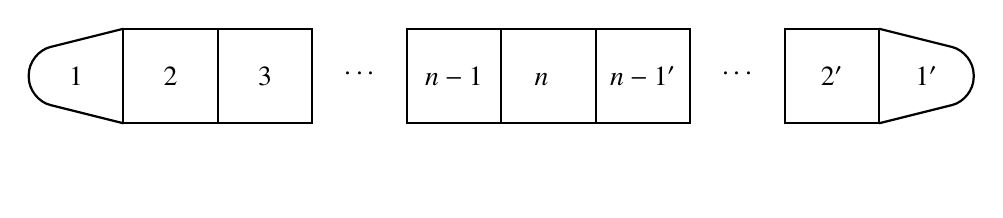
\begin{tikzpicture}[>=angle 90,scale=1.2]
\draw[thick] (1,0) -- (3,0) -- (3,1) -- (1,1) --cycle;
\draw[thick] (4,0) -- (7,0) -- (7,1) -- (4,1) --cycle;
\draw[thick] (8,0) -- (9,0) -- (9,1) -- (8,1) --cycle;
\draw[thick,rounded corners=8pt] (1,0) -- (0,0.25) -- (0,0.75)-- (1,1);
\draw[thick,rounded corners=8pt] (9,0) -- (10,0.25) -- (10,0.75)-- (9,1);
\draw (0.5,0.5) node {$1$};
\draw (1.5,0.5) node {$2$};
\draw (2.5,0.5) node {$3$};
\draw (3.5,0.5) node {$\cdots$};
\draw (4.5,0.5) node {$n-1$};
\draw (5.5,0.5) node {$n\phantom{1}$};
\draw (6.5,0.5) node {$n-1'$};
\draw (7.5,0.5) node {$\cdots$};
\draw (8.5,0.5) node {$2'$};
\draw (9.5,0.5) node {$1'$};
\foreach\x in {2,5,6}
\draw[thick](\x,0)--(\x,1);
\draw[white] (0,-0.7);
\end{tikzpicture}
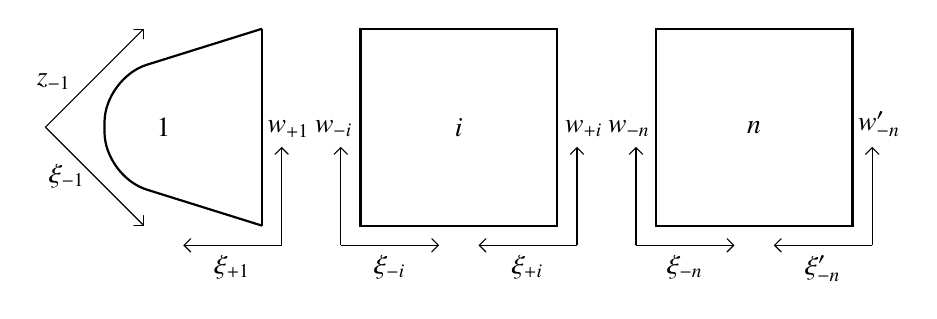
\begin{tikzpicture}[>=angle 90,scale=2.5,yshift=1cm]
\draw[thick,rounded corners=16pt] (1,0) -- (0.2,0.25) -- (0.2,0.75)-- (1,1);
\draw[thick] (1,0) -- (1,1);
\draw[thick] (1.5,0) -- ++(1,0) -- ++ (0,1) -- ++ (-1,0) -- cycle;
\draw[thick] (3,0) -- ++(1,0) -- ++ (0,1) -- ++ (-1,0) -- cycle;
\draw (0.5,0.5) node {$1$};
\draw (2,0.5) node {$i$};
\draw (3.5,0.5) node {$n$};
%box1
\draw[->,xshift=-0.1cm] (0,0.5) -- node[above,left]{$z_{-1}$\phantom{1}} ++(0.5,0.5);
\draw[->,xshift=-0.1cm] (0,0.5) -- node[below,left]{$\xi_{-1}$} ++(0.5,-0.5);
\draw[->,xshift=0.1cm,yshift=-0.1cm] (1,0) -- ++(0,0.5) node[right,above]{\phantom{1}$w_{+1}$};
\draw[->,xshift=0.1cm,yshift=-0.1cm] (1,0) -- node[below]{$\xi_{+1}$} ++(-0.5,0) ;
%box2
\draw[->,xshift=-0.1cm,yshift=-0.1cm] (1.5,0) -- ++(0,0.5) node[above]{$w_{-i}$\phantom{1}};
\draw[->,xshift=-0.1cm,yshift=-0.1cm] (1.5,0) -- node[below]{$\xi_{-i}$} ++(0.5,0) ;
\draw[->,xshift=0.1cm,yshift=-0.1cm] (2.5,0) -- ++(0,0.5) node[above]{\phantom{1}$w_{+i}$};
\draw[->,xshift=0.1cm,yshift=-0.1cm] (2.5,0) -- node[below]{$\xi_{+i}$} ++(-0.5,0) ;
%box3
\draw[->,xshift=-0.1cm,yshift=-0.1cm] (3,0) -- ++(0,0.5) node[above]{$w_{-n}$\phantom{1}};
\draw[->,xshift=-0.1cm,yshift=-0.1cm] (3,0) --  node[below]{$\xi_{-n}$} ++(0.5,0);
\draw[->,xshift=0.1cm,yshift=-0.1cm] (4,0) -- ++(0,0.5) node[above]{\phantom{1}$w'_{-n}$};
\draw[->,xshift=0.1cm,yshift=-0.1cm] (4,0) -- node[below]{$\xi'_{-n}$} ++(-0.5,0);
\end{tikzpicture}

\caption{Local Coordinates on $S$}
\end{figure}

%\diabox{XX \centerline{Diagram 1.  Local Coordinates on $S$}}{3 truein}{diag1.ps}

\medskip

We will treat the irreducible components $S_1,\ldots,S_n$.
The remaining components are treated in an identical manner,
by adding primes to all of the coordinates.  We set
\begin{align*}
x_{-i} &= {w_{-i}\over (1-t_i w_{-i} )},\ \ \ \ \,\,
y_{-i}  = {\xi_{-i}\over
  (1+t_1 x_{-i} )\cdots (1+t_i x_{-i} )},\ \text{ for }1<i\le n,\\
x_{+i} &= {w_{+i}\over (1-t_{i+1} w_{+i})},\ \ 
y_{+i} = {\xi_{+i} (1+t_1 x_{+i})\cdots (1+t_i x_{+i})},\ \text{ for }
 1\le i<n.\\
\end{align*}

Transporting the action of the Weyl group (described in
[H2,VI,Theorem 1.6]) to this new set of coordinates, 
we find that the coordinates $x_{\pm i}, y_{\pm i}$ are all
Weyl-group invariant.  (To verify this, one must know explicit
values for the constants $e(\alpha,\beta)$:
$e(\alpha_i,\alpha_{i+1}) = 1$, $e(\alpha_{i},\alpha_{i-1})=
-1$, for $i<n$,  and $e(\alpha_n,\alpha_{n-1}) = -2$.)
We may also take $\zeta=1$, since $\text{SO}(2n+1)$ is quasisplit.
The transition relations of
[H2,V,Lemma 5.3,Lemma 6.1] imply that on the overlap of
two coordinate charts on $S_i$, we have
$x_{-i} = x_{+i}$ and $y_{-i} y_{+i}=1$, for $i<n$.
On $S_n$, we have $x_{-n} = -x_{-n}'$ and $y_{-n} y_{-n}' = 1/P(x_{-n})$,
where $P(x_{-n}):= (1-t_1^2 x_{-n}^2)\cdots (1-t_n^2 x_{-n}^2)$.

The
Galois group $\Gal(\bF/F)$ permutes the irreducible
components of ${\mathcal B}_u$ and $S$ in a compatible way.  For
$\text{SO}(2n+1)$ and the unipotent class associated with $a\,F^{\times\,2}$,
each irreducible component is defined over $E=F(\sqrt{a})$.  

Now consider a nontrivial coset $a\,F^{\times\,2}$.
In this case,
only one
irreducible component $S_n$ of $S$ contains rational points.
The action of the nontrivial element $\sigma_0$ in
the Galois group $\Gal(E/F)$ on the coordinates
is $\sigma_0(x_{-n}) = -x_{-n}$ and 
$\sigma_0(y_{-n}) y_{-n} = 1/P(x_{-n})$. 
(See [H2,VI,Theorem 1.6].
There is a sign error in part (d) of that theorem:
the right-hand side of the formula for $\sigma_0(w)$
should be negated.)
The coordinates are Weyl-group invariant, so that these
relations hold for all Cartan subgroups.
The Shalika germ is then the integral over the surface $S_n$
with respect to the measure $|x_{-n}^{-2} y_{-n}^{-1} dx_{-n} dy_{-n}|$.
Since $\sigma_0(y_{-n}) y_{-n} = 1/P(x_{-n})$, we see that $P(x_{-n})$
is a norm from $E$, so that
$$1 = {1\over 2} (1 + \eta(P(x_{-n}))).$$
We may also replace $y_{-n}$ by a multiple of $y_{-n}$ so that
its norm is $1$, independent of $x_{-n}$.
Thus the germ is
$$\int_{S_n} \left| {dy_{-n}\, dx_{-n}\over y_{-n}\,\, x_{-n}^2}\right|
= {1\over 2} \int\left | {dy_{-n}\over y_{-n}}\right|
 \int_{\Imm}\left | dx_{-n}\over x_{-n}^2 \right| +
 {1\over 2} \int\left | {dy_{-n}\over y_{-n}}\right|
 \int_\Imm \eta(P(x_{-n}))\left | dx_{-n}\over x_{-n}^2 \right|.$$
By Lemma 2.2, the integral $\int |dx_{-n}/x_{-n}^2|$ is zero,
so that the first of the two terms is zero.  The normalizing
factor $\int |dy_{-n}/y_{-n}|/2$ is independent
of $x_{-n}$ and $t_i$.  Ignoring this constant,
we obtain the formula of the theorem.

Now turn to the trivial coset $F^{\times\,2}$.  Each
irreducible component is defined over $F$.
We must compute the volume of the surface with respect to
the given coordinates and the measure attached to the differential form
$${d x_{-i} \wedge dy_{-i}\over x_{-i}^2 \,\,y_{-i}}.$$
The coordinates $x_{\pm i}$, $y_{\pm i}$
are defined over $F$
for every Cartan subgroup, because the 
coordinates are Weyl-group invariant.
The form has a simple pole along each intersection of adjacent
irreducible components. 
One way to compute
the volume is to pick coordinates in such a way that the
only contributions to volume come from the poles.  With
the coordinates given above, the only contribution to
volume will come from the irreducible component $S_n$.

We begin this calculation by showing that the contribution
of each simple pole $\xi_{-i}=0$, for $i>1$,  is zero.  We follow
the procedure and notation explained in [H2,p83] (compare
[La,p469] and [H1,p238]).  
By [H2,V,6.1.d], on the irreducible component $S_i$,
the coordinate
$y_{-i}$ is the restriction of
$${z(W_+,\alpha_i)\over (t_i-t_{i+1}) w_{-i} e(\alpha_i,\alpha_{i-1})(1+t_1 x_{-i})
\cdots (1+t_i x_{-i} )},$$
and $y_{+(i-1)}$ is the restriction of
$${z(W_+,\alpha_{i-1}) (1+t_1 x_{+(i-1)})\cdots (1+t_{i-1} x_{+(i-1)})\over
(t_{i-1}-t_i) w_{+(i-1)} e(\alpha_{i-1},\alpha_i)}.$$
Along the pole, $w_{-i}=w_{+(i-1)}$, $x_{-i} = x_{+(i-1)}$, 
and the product $y_{-i}y_{-i}$ is the restriction
of 
\begin{equation}{z(W_+,\alpha_i)z(W_+,\alpha_{i-1})\over
(t_i-t_{i+1})(t_{i-1}-t_i) w^2 e(\alpha_i,\alpha_{i-1})e(\alpha_{i-1},\alpha_i)
(1+t_i x_{-i})}.\tag{1.3}
\end{equation}
For the definitions of $\lambda$, $z(W_+,\alpha)$, and so forth
we refer the reader to [H2].
The quotient of $\lambda$ by Expression 1.3 simplifies to
$$ x(\gamma)w_{-i}(1+t_i x_{-i} ) = x(\gamma) x_{-i}.$$
We must then integrate the logarithm of the absolute value 
of this quotient 
over the pole $\xi_{-i}=0$ of $S_i$ using the differential
form $d x_{-i}/x_{-i}^2$. Both $x(\gamma)$ and
$x_{-i}$ are defined over $F$.  It then follows from the
vanishing of the integrals
$$\int_F \log|x| \left | {dx\over x^2}\right|,\qquad
  \int_F \left| {dx\over x^2}\right |$$
that the simple poles contribute nothing to the principal-value
integral.

Next we analyze the contributions from the remainder of the
irreducible components $S_i$, $i\ne 1,n$.  The contribution
is obtained by truncating near the simple poles:
$|y_{-i}|\ge \epsilon_1$, $|y_{+i}|\ge \epsilon_2$.
As we have $y_{+i}=1/y_{-i}$, we find that the contribution
is (by Lemma 2.2)
$$\int_{\epsilon^{-1}_2 \ge |y_{-i}|\ge \epsilon_1}
\left| {dy_{-i}\over y_{-i}}\right |
\int_F \left| { dx_{-i}\over x^2_{-i}}\right| =
\int_{\epsilon^{-1}_2 \ge |y_{-i}|\ge \epsilon_1}
\left| {dy_{-i}\over y_{-i}}\right | \cdot 0 = 0.$$

The irreducible component $S_1$ requires special treatment.
On $S_1$ the coordinates $(z_{-1},\xi_{-1}) = (z,\xi)$
are essentially the $F$-variables $x_0 = x_{+1}/y_{+1}$
and $y_0 := 1/y_{+1}$.  The form is $x_0^{-2} dx_0\wedge dy_0$.
The component $S_1$ makes no contribution because the truncated
integral $\int_{|y_0|< C} |x_0^{-2} dx_0\,dy_0|$ is zero.
(Compare [H1,page237] where this argument is made in the
rank two situation.)

The final contribution comes from the truncated integral on $S_n$.
Here we truncate by $|y_{-n}|\ge \epsilon_1$ and $|y'_{-n}|\ge \epsilon_2$.
Since $y_{-n}y_{-n}' = 1/P(x_{-n})$, we have a contribution
$$
\int_{(\epsilon_2 |P(x_{-n})|)^{-1} \ge |y_{-n}|\ge \epsilon_1}
\left| {dy_{-n}\over y_{-n}} \right |
\int_F \left|{dx_{-n}\over x_{-n}^2}\right |,$$
and this is a constant times
$$\int_F \log|P(x_{-n})| \left|{dx_{-n}\over x_{-n}^2}\right|.$$
This completes the proof of Theorem 1.2.
\end{proof}

\section{The Basic Identity for the Subregular Germs}
%\vfill\break
%\centerline{\headfont Section 2.  The Basic Identity for the Subregular Germs.}
%\bigskip

\noindent
{\bf Notation.}\  
Throughout the remainder of this paper,
let $F$ be a $p$-adic field of characteristic
zero, of odd residual characteristic with fixed
algebraic closure $\bF$.  Let $O_F$
denote the ring of integers in $F$, and let $\pi$ denote
a uniformizing element in $F$.
We often work with
a fixed finite Galois extension $K/F$, with intermediate
fields $E$, $E_1$, and so forth. 
Let $|\cdot|$ denote
the normalized absolute value on $F$, extended to the
field $K$.  Define $\val(x)$, for $x\in K$, by $|x| = q^{-\val(x)}$,
where $q$ is the cardinality of the residue field of $F$.  
Thus $\val(x) e(K/F) \in \Z$, for $x\in K$, 
where $e(K/F)$ is the
ramification index of the field extension $K/F$.  We define
$\log|x|$ to be $-\val(x)$.

We introduce further notation for this particular section.
We enumerate the
nontrivial quadratic extensions $E_1$, $E_2$, $E_3$ of $F$,
selecting $E_1$ to be the unramified extension, and $E_2$, $E_3$
to be ramified.  We select uniformizing elements $\pi_2\in E_2$
and $\pi_3\in E_3$.  We may assume that $\pi_2^2 = \pi$, a fixed
uniformizing element of $F$, and that $\pi_3^2 = \epsilon\pi$,
where $\epsilon$ is a unit in $F$.  Then $E_1$ is obtained by
adjoining to $F$ a square root of $\epsilon$.  The Galois
groups $\Gal(E_i/F)$ of these quadratic extensions have nontrivial
elements that we denote $\sigma_i$, for $i=1,2,3$.  The quadratic
extensions have {\it imaginary} axes $\Imm_i = \{u\in E_i| \sigma_i(u) = -u\}$,
for $i=1,2,3$.  We let $\eta_i$ be the 
quadratic character of $F^\times$
associated with $E_i$, for $i=1,2,3$.  We have $\pi_i\in \Imm_i$,
for $i=2,3$.

For $a,b\in F$, we let $P(x) = P(x,a,b)$ denote the polynomial
$P(x) = 1-ax^2 + bx^4$.  We factor the polynomial as
$P(x) = (1-\alpha x^2)(1-\beta x^2)$, where $\alpha=\alpha(a,b)$,
$\beta=\beta(a,b)$ lie in some quadratic extension of $F$.
We define a dual polynomial 
\begin{align*}
P'(x,a,b) &= P(x,2a,a^2-4b) = 1-2ax^2 + (a^2-4b)x^4 = (1-a'x^2 + b'x^4)\cr
	  &= (1-(\alpha^{1/2} - \beta^{1/2})^2x^2)
                (1-(\alpha^{1/2}+\beta^{1/2})^2x^2)\cr
	  &= (1-\alpha'x^2)(1-\beta'x^2),
\end{align*}
where $\alpha' = \alpha+\beta-2\sqrt{b} = a-2\sqrt{b}$, and
$\beta' = \alpha+\beta+2\sqrt{b} = a+2\sqrt{b}$.  Also,
$a'=2a$, $b'=a^2-4b = \alpha'\beta'=(\alpha-\beta)^2$.
The constants $a,b,a',b',\alpha,\beta,\alpha',\beta'$ will 
satisfy these fixed relations throughout the section.

We consider the one-form $dx$ on the affine line and the associated
measure $|dx|$ on $F$.  We set
$$\Gamma_0(a,b) = \int_{F} \log|P(x,a,b)| \leftdx.$$
This and all the integrals that follow  are
to be interpreted as a principal-value integrals.
Extending the absolute value $|\cdot|$ and the associated measure
to field extensions $E_i/F$, we also set
$$\Gamma_i(a,b) = \int_{\Imm_i} \eta_i(P(u,a,b))\leftdu.$$
We normalize these integrals by setting $\bGamma_i(a,b) =
\Gamma_i(a,b)/\Gamma_i(\epsilon,0)$, for $i=0,1,2,3$.
We have seen that these integrals are the stable
subregular Shalika germs of $\text{SO}(5)$.
The integrals $\Gamma_2$ and $\Gamma_3$ are {\it elliptic} in the
sense that for certain choices of parameters $a,b\in F$ the values
of the integrals are expressed by the number of points on elliptic
curves over finite fields.

Set $s_q = 1$, if $-1$ is a square in $F$, and set $s_q=-1$ otherwise.

We are now ready to state the main technical result of this paper.  
By Theorem 1.2, this result implies the matching of stable
subregular Shalika germs.
It expresses
the nontrivial part of the transfer of Shalika
germs from the twisted reductive groups $GL(4)$ and $GL(5)$ to 
endoscopic groups $\text{SO}(5)$ and $\text{Sp}(4)$.  The geometrical
content of this proposition is the existence of particular isogenies of
elliptic curves.
\bigskip

\noindent
\begin{cthm}{Proposition 2.1}  For all $a,b\in F$,
$$\begin{pmatrix}\bGamma_0(2a,a^2-4b) \\
          \bGamma_1(2a,a^2-4b) \\
          \bGamma_2(2a,a^2-4b) \\
          \bGamma_3(2a,a^2-4b) \end{pmatrix}
= {1\over 2}
\begin{pmatrix}1&1&1&1\\
        1&1&-1&-1\\
        1&-1&s_q&-s_q\\
        1&-1&-s_q&s_q\end{pmatrix}
\begin{pmatrix}\bGamma_0(a,b)\\
        \bGamma_1(a,b)\\
        \bGamma_2(a,b)\\
        \bGamma_3(a,b)\end{pmatrix}.
$$
\end{cthm}

This proposition expresses a duality in the sense that the statement
is equivalent to the identity
$$\begin{pmatrix}\bGamma_0(a,b) \\
          \bGamma_1(a,b) \\
          \bGamma_2(a,b) \\
          \bGamma_3(a,b) \end{pmatrix}
= {1\over 2}
\begin{pmatrix}1&1&1&1\\
        1&1&-1&-1\\
        1&-1&s_q&-s_q\\
        1&-1&-s_q&s_q\end{pmatrix}
\begin{pmatrix}\bGamma_0(2a,a^2-4b)\\
        \bGamma_1(2a,a^2-4b)\\
        \bGamma_2(2a,a^2-4b)\\
        \bGamma_3(2a,a^2-4b)\end{pmatrix},
$$
obtained by taking the inverse of the $4\times 4$ matrix.  We could
also substitute $a'$ for $a$ and $b'$ for $b$ and note that
$\bGamma_i(2a',a^{\prime\,2} - 4b') = \bGamma_i(4a,16b) = \bGamma_i(a,b)$
because $|2|=1$. Note that the $4\times 4$ matrix is the
matrix $\eta_i(x_j)$ obtained by pairing the trivial character
$\eta_0$ and the nontrivial characters
$\eta_1$, $\eta_2$, $\eta_3$ with the
representatives $x_j = 1,\epsilon,\pi,\epsilon\pi$
of the cosets of $F^\times/F^{\times\,2}$.


The proposition is
proved by calculating the integrals on both sides for all possible
choices of parameters $a,b\in F$, and comparing the two sides.
We will see that the integrals $\bGamma_i(a,b)$ are linearly
independent over ${\mathbb C}$, so that the $4\times4$ matrix in
the proposition is unique.

The most difficult of these integrals to compute are $\Gamma_i(a,b)$,
for $i=2,3$.  In the typical case, $|\alpha|=|\beta|=|\alpha-\beta|$.
Let us briefly describe how it is calculated, say for $i=2$.  There
will be a large number of integrals such as this to compute, and
we will leave the routine details of the calculations to the reader.
Under the substitution $u=\pi_2x$, the
integral becomes
$$|\pi_2|^{-1}\int_{F}\eta_2(P(x,\bar a,\bar b))\leftdx,$$
where $\bar a = \pi_2^{2} a$, $\bar b = \pi_2^{4} b$, $\bar \alpha
=\pi_2^{2} \alpha$, and $\bar \beta = \pi_2^{2}\beta$.

On the interval
$|\bar\alpha x^2| >1$, we have $\eta_2(P(x,\bar a,\bar b)) 
        = \eta_2(\bar b)$, a constant,
and the integral becomes a simple geometric series.
On the interval $|\bar\alpha x^2| <1$, we have $\eta_2(P(x,\bar a,\bar b)) = 1$,
and again we have a geometric series that is easily summed.
On the set $\{x: \ |\bar \alpha x^2| = 1; \ |P(x,\bar a,\bar b)| = 1\}$,
we see that $\eta_2(P(x,\bar a,\bar b))$ depends only on whether the
reduction to the residue field of $P(x,\bar a,\bar b)$ is a square,
so the integral will be expressed in
terms of the number of affine
points (with $\bar y\ne 0$) 
on the curve over the finite field $\bar y^2 = \bar P(\bar x)$,
obtained by reducing $P(x,\bar a,\bar b)$.  
This explains the appearance of 
elliptic curves.  

Finally we must consider elements $x$
such that $|\bar \alpha x| = 1$ and $|P(x,\bar a,\bar b)|<1$.
Call this the set of {\it approximate roots}.
We have a local coordinate $t = \bar \alpha(x-x_0)$, with $|t|<1$,
near a fixed approximate root $x_0$.  The integral is a constant times
$$\int_{|t|<1} \eta_2(t)|dt|,$$
and this is zero because $\eta_2$ is ramified.  So the set of
approximate roots contributes nothing to the integral.  When
we use the unramified character $\eta_1$, however, there is in
general a nonzero contribution from the set of approximate roots.
See Lemma 2.6.

The following vanishing result, which we have already invoked
more than once, will be used frequently in this paper.  A proof
is found in [LS1].

\bigskip
\noindent
\begin{cthm}{Lemma 2.2} Let $\theta:F^\times\to \C^\times$ be a
nontrivial quasicharacter of $F^\times$.  Then
$$\int_{\bP^1} \theta(x) \left | {dx\over x}\right | =0.$$
\end{cthm}

It is often easier to compute the integral of $\eta_i(P) - 1$ 
than the integral of $\eta_i(P)$.  The two integrands give the
same result because of the lemma.
If, for example, $\eta_2(\bar b) = 1$, then $\eta_2(P(x,\bar a,\bar b))-1=0$,
except when $|\bar\alpha x^2|=1$, so that the only contributions to the
integral come from the curve over the finite field.

Rather than show the calculation of all of the integrals, we will
show how to express them in terms of integrals whose values
have been tabulated.
The following integrals are tabulated in the appendix.
$$\LOG(a) := \int_{F} \log|1-ax^2| \leftdx,
\quad \text{ for } a\in F.$$
$$H_i(a):= \int_{F}\eta_i(1-ax^2) \leftdx,
\quad \text{ for } a\in F \text{ and } i=1,2,3.$$
In terms of these integrals, the normalizing constants
entering into the definitions of the functions $\bGamma_i(a,b)$
are
$\Gamma_0(\epsilon,0) = \LOG(\epsilon)$, $\Gamma_1(\epsilon,0) = H_1(1)$,
$\Gamma_2(\epsilon,0) = H_2(\epsilon \pi_2^2)/|\pi_2| = \sqrt{q}H_2(\epsilon\pi)$,
$\Gamma_3(\epsilon,0) = \sqrt{q} H_3(\pi)$.  
Thus, by the tables in the appendix,
the normalized integrals $\bGamma_i(a,b)$ stand in explicit relation
to $\Gamma_i(a,b)$.

\bigskip
\noindent
\begin{cthm}{Lemma 2.3}  It is enough to establish the Proposition 2.1 
in the following
four cases.  %\parskip=0pt \parindent=0pt
\begin{enumerate}[label=(\arabic*)]
\item $|\alpha|>|\beta|$, and $\alpha,\beta\in F$.
\item $|\alpha|=|\beta| = |\alpha-\beta|=|\alpha'|=|\beta'|=|\alpha'-\beta'|$,
and $\val(\alpha)\in {\mathbb Z} + {1\over 2}$.
\item $|\alpha|=|\beta| = |\alpha-\beta|=|\alpha'|=|\beta'|=|\alpha'-\beta'|$,
and $\val(\alpha)\in 2{\mathbb Z}$.
%
\item $|\alpha|=|\beta| = |\alpha-\beta|=|\alpha'|=|\beta'|=|\alpha'-\beta'|$,
and $\val(\alpha)\in 2{\mathbb Z}+1$.
\end{enumerate}
\end{cthm}

\noindent
\begin{proof}  First we dispense with the degenerate case when $\beta=0$.
It is easily deduced from the tables of the appendix that $\bGamma_i(a,0)$
is independent of $i$.  The proposition reduces to the vanishing integral
of Lemma 2.2 and the claim
$$\bGamma_0(2a,a^2) = 2\bGamma_0(a,0).$$
This is an immediate consequence of the identity
$\log|1-2a x^2+a^2 x^4| = 2\log|1-a x^2|$.
Thus we assume that $\beta\ne0$, by symmetry that $\alpha\ne0$,
$b\ne 0$, and, by the duality following the statement of
Proposition 2.1, that $\alpha'\ne0,\beta'\ne0$, 
and $b'=(\alpha-\beta)^2\ne0$.

Since $\alpha$ and $\beta$ are the roots of a quadratic
polynomial over $F$, if the roots are not in $F$, then their valuations
are equal.  If $|\alpha|\ne |\beta|$, then by symmetry we may take
$|\alpha|>|\beta|$.

Now assume that $|\alpha|=|\beta|$.  If $|\alpha'|\ne |\beta'|$, then
by symmetry we can assume that $|\alpha'|>|\beta'|$, and then by
the duality explained after the 
statement of the proposition, we may conclude the
proposition from Case 1.  So we may assume that 
$\alpha^{\prime\,1/2} = (\alpha^{1/2}-\beta^{1/2})$ and 
$\beta^{\prime\,1/2} = (\alpha^{1/2}+\beta^{1/2})$ have equal valuations.
Their valuation must equal that of either their sum or difference,
so $|\alpha^{1/2}-\beta^{1/2}| = |\alpha^{1/2}+\beta^{1/2}| = |\alpha^{1/2}|
= |\beta^{1/2}|$.  Thus, $|\alpha|=|\beta|=|\alpha-\beta| =
|\alpha'|=|\beta'| = |\alpha'-\beta'|$.   Now Cases 2, 3, and 4 give
the three possibilities for the valuation of an element in a quadratic
extension of $F$.
\end{proof}


\bigskip
\centerline{\bf Subregular Case 1. Unequal Valuation.}
\bigskip

We now check Proposition 2.1 in Case 1 : $|\alpha| >|\beta|$, and $\alpha,
\beta\in F$.  Dropping subscripts, we let $\eta$ be a quadratic character
associated with a quadratic extension $E$, and let $\Imm$ be the
imaginary axis of $E$.

\bigskip
\noindent
\begin{cthm}{Lemma 2.4}  Suppose that $|\alpha|>|\beta|$, with $\alpha,\beta\in F$.
Then
$$\int_{F} \log|(1-\alpha x^2)(1-\beta x^2)| \leftdx
  = \LOG(\alpha) + \LOG(\beta), $$
and
$$\int_{\Imm} \eta((1-\alpha u^2)(1-\beta u^2))\leftdu
  = \int_{\Imm}\eta(1-\alpha u^2) \leftdu +
\eta(\alpha) \int_{\Imm}\eta(1-\beta u^2)\leftdu.$$
\end{cthm}

\bigskip
\begin{proof}  The first statement follows immediately from the identity
$\log|xy| = \log|x|+\log|y|$, and the definition of the integral $\LOG$.
On the interval $|u|^2 < 1/|\beta|$, we have $\eta(P(u)) = \eta(1-\alpha u^2)$,
and $\eta(\alpha)=\eta(\alpha)\eta(1-\beta u^2)$.  
And on the interval
$|u|^2 \ge 1/|\beta|$, we have $\eta(P(u)) = \eta(\alpha)\eta(1-\beta u^2)$,
and $\eta(\alpha)=\eta(1-\alpha u^2)$.  Thus 
$$\eta(P(u)) + \eta(\alpha) = \eta(1-\alpha u^2) + \eta(\alpha)\eta(1-\beta u^2),$$
for all $u\in \Imm$.  Now integrate over the imaginary axis, and use Lemma 2.2
to complete the proof: $\int_{\Imm} \eta(\alpha) |du/u^2|=0$.
\end{proof}

With a parametrization of the imaginary axis by $u = cx$, for some 
fixed $c\in \Imm$
and $x\in F$, the integrals on the right-hand side 
in Lemma 2.4 equal those tabulated
in the appendix.  Thus, the integrals $\bGamma_i(a,b)$ in Case 1
are known functions
of $q$.

Now we turn to the dual direction.  Recall that $P'(x) = (1-2ax^2+(a^2-4b)x^4)
= (1-\alpha'x^2)(1-\beta'x^2)$.  The first case of Proposition 2.1
is a direct 
consequence of the following lemma and the previous one, because
together they give explicit formulas for the functions $\bGamma_i$.
We leave the details of
the verification to the reader.

\bigskip
\noindent
\begin{cthm}{Lemma 2.5}  Suppose that $|\alpha|>|\beta|$, and that $\alpha,\beta\in F$.
Then
\parskip=0pt

(1)  $\int_{\Imm}\eta(P'(u)) |du/u^2| = 0$, if $\alpha^{1/2}\not\in\Imm$.

(2)  $\int_{\Imm}\eta(P'(u)) |du/u^2| = 2\int_{\Imm}\eta(1-\beta u^2)|du/u^2|$,
       if $\alpha^{1/2}\in \Imm$.

(3)  $\int_{F}\log|P'(x)| |dx/x^2| = 2\int_{F}
        \log|1-\alpha x^2| |dx/x^2|$,
       if $\alpha\not\in F^{\times\,2}$.

(4) $\int_{F}\log|P'(x)| |dx/x^2| = 2\int_{F}\log|1-\beta x^2|
     |dx/x^2|$, if $\alpha\in F^{\times\,2}$.
\end{cthm}

\bigskip
\noindent
\begin{proof} Since $\alpha'=(\alpha^{1/2}-\beta^{1/2})^2$, and $|\alpha|>|\beta|$,
we have $|\alpha'| = |\alpha|$.  Similarly, $|\beta'| =|\alpha|$.  So
$|\alpha'|=|\beta'|$.  On the interval $|u|^2 < 1/|\beta'|$,
we see that $\eta(P'(u)) = 1$, and on the interval $|u|^2 > 1/|\beta'|$,
we see that $\eta(P'(u)) = \eta(b') = 1$, since $b'=(\alpha-\beta)^2\in
F^{\times\, 2}$.

On the set $\{u:\ |u|^2 = 1/|\beta'|,\text{ and }|P'(u)|=1$\},
we see that $\eta(P'(u)) = \eta((1-\alpha u^2)^2) = 1$.
So $\eta(P'(u)) = 1$, for all $u\in \Imm$, except at points $u$
in the imaginary axis such that $|1-\alpha u^2|<1$.  There are
no such points if $\alpha^{1/2}\not\in\Imm$.  
In this case, the integral of Part 1 of the lemma is 
equal to $\int_{\Imm} |du/u^2|$ and hence is zero by Lemma 2.2.

Assume that $\alpha^{1/2}\in \Imm$.  The integral of Part 2
the lemma is equal to 
$$\int _{|1-\alpha u^2|<1} \eta(P'(u)) -1 \leftdu.$$
Write $x \sim y$ if $xy^{-1}\in F^{\times\,2}$.
If $|x-y|<1$ and $|x|\ge 1$, for $x,y\in F$, 
then $x\sim y$.

We have
$P'(u) = ((1- \alpha^{1/2} u)^2-\beta u^2)
((1+\alpha^{1/2} u)^2-\beta u^2)$.  Thus
if $|1-\alpha^{1/2} u|<1$,
then $P'(u) \sim ((1-\alpha^{1/2}u)^2-\beta u^2)2^2
\sim (1-\beta v^2)$, where $v = u/(1-\alpha^{1/2}u)$.  Similarly, if
$|1+\alpha^{1/2} u|<1$,
then $P'(u)\sim (1-\beta v^{\prime\,2})$,
where $v' = u/(1+\alpha^{1/2} u)$.
Making this change of coordinates we have
$$\int_{|1-\alpha u^2|<1} \eta(P'(u))-1 \leftdu = 2
\int_{\Imm} \eta(1-\beta v^2)-1 \leftd v.$$
We have used the fact that $v$ and $v'$ make equal contributions to the
integral.  We have also used the fact that $|1-\alpha^{1/2} u | <1$
if and only if $|1+\alpha^{1/2} v  |$, or equivalently $|\alpha^{1/2}v|$,
is greater than 1.  But if $|\alpha^{1/2} v|\le 1$, then $1-\beta v^2\sim 1$,
so the integrand vanishes.  This justifies the integration over the
full imaginary axis.  Part 2 now follows from Lemma 2.2.

Now turn to the log terms.  We easily check that 
\begin{align*}
\int_{F} |P'(x)|\leftdx &= \int_{|\beta'x^2|>1} \log|b'x^4|\leftdx
        + \int_{|\beta'x^2|=1,\ |P'(x)|<1} \log|P'(x)|\, \leftdx\\
 &= 2\int_{|\alpha x^2| >1} \log|\alpha x^2| \leftdx 
        + \int_{|\beta'x^2|=1,\ |P'(x)|<1} \log|P'(x)|\, \leftdx.
\end{align*}
If $\alpha$ is not a square, the first term is 
$2\int_{F} \log|1-\alpha x^2| |dx/x^2|$, and the second term is
zero.  This proves Part 3 of the lemma.  Now assume that $\alpha$ is
a square.  Under the obvious symmetry $\alpha^{1/2} \leftrightarrow
-\alpha^{1/2}$, we have
$$\int_{|\beta'x^2|=1,\   |P'(x)|<1} \log|P'(x)|\,\leftdx =
   2|\alpha|\int_{|1+\alpha^{1/2} x|<1} \log|P'(x)| \,|dx|.$$
If we set $v=x/(1+\alpha^{1/2} x)$, then
whenever $|1+\alpha^{1/2}x|<1$ we have
$$\log|P'(x)| = \log|2^2 ((1+\alpha^{1/2} x)^2 - \beta x^2)| = 
2\log|1+\alpha^{1/2}x| + \log|1-\beta v^2|.$$
The integral of the second term is $2\int_{F}\log|1-\beta v^2| \,|dv/v^2|$.
The integral of the first term becomes
$-2\int_{F} \log |1-\epsilon \alpha t^2| \,|dt/t^2|$, under the
substitution $1+\alpha^{1/2} x = 1/(t \alpha^{1/2})$.  The result
follows.
\end{proof}

\bigskip
\centerline{\bf Subregular Case 2.  ${1\over 2}$-Integral Valuation.}
\bigskip

Next we check the proposition in Case 2: $\val(\alpha)\in {\mathbb Z}+{1\over 2}$.
The root
$\alpha$ lies in a ramified quadratic extension of $F$.  
If $\alpha\in E_2\setminus F$, then $b\in -\pi \,F^{\times\,2}$,
and if $\alpha\in E_3\setminus F$, then $b\in -\pi\epsilon\,F^{\times\,2}$,
so the quadratic field containing $\alpha$ is determined by the
class of $b$ in $F^\times/F^{\times\,2}$.
Case 2 of Proposition 2.1 is a direct consequence of Part 3 of
the following lemma.


\bigskip
\noindent
\begin{cthm}{Lemma 2.6}
(1)  If $b\in -\pi\epsilon\,F^{\times\,2}$, then
\begin{align*}
\Gamma_0(a,b) &= {|b\pi^{-1}|^{1/4}(3q+1)\over q(q-1)}, \text{ if }
			\val(b)\equiv 1 \mod 4,\\
\Gamma_0(a,b) &= {|b\pi^{-3}|^{1/4}(q+3)\over q(q-1)}, \text{ if }
			\val(b)\equiv 3 \mod 4,\\
\Gamma_1(a,b) &= {-2|b\pi^{-j}|^{1/4}\over q}, \text{ if }
			\val(b)\equiv j \mod 4 \text{ and } j=1, 3,\\
\Gamma_2(a,b) &= {-2|b\pi^{-1}|^{1/4}\sqrt{q}\over q}, \text{ if }
			\val(b)\equiv 1 \mod 4,\\
\Gamma_2(a,b) &= {-2|b\pi^{-3}|^{1/4}\sqrt{q}\over q^2}, \text{ if }
			\val(b)\equiv 3 \mod 4,\\
\Gamma_3(a,b) &= 0.
\end{align*}
\smallskip

(2)  If $b\in -\pi\,F^{\times\,2}$, then the same relations
hold after interchanging the subscripts $2$ and $3$ in Part 1.


\smallskip
(3)

\begin{align*}
\Gamma_i(2a,a^2-4b) &= \Gamma_i(a,b), \text{ for } i=0,1,\\
\Gamma_i(2a,a^2-4b) &= \Gamma_i(a,b), \text{ for } i=2,3, \text{ if }
		-1 \text{ is a square,}\\
\Gamma_i(2a,a^2-4b) &= \Gamma_j(a,b), \text{ for } (i,j) = (2,3), (3,2),
		\text{ if } -1 \text { is not a square.}
\end{align*}

\end{cthm}

\smallskip

\noindent
\begin{proof}
The integrals of Part 1 are easily computed. 
Assume 
$\alpha\in E_3\setminus F$.  
If $u\in \Imm_3$, then $P(u)$ is
the norm of $(1-\alpha u^2)$, so that $\eta_3(P(u)) = 1$,
and $\Gamma_3(a,b)=0$ by Lemma 2.2.
The other integrals quickly reduce to geometric series and the
integrals of the appendix.
 We omit the details.
We show that Parts 1 and 2 imply Part 3.
Note that
$\Gamma_i(a,b)$ is independent of $a$ and depends only on $b$ modulo
the multiplicative group of the squares of units, 
and that $\Gamma_0$ and $\Gamma_1$ depend only on the
valuation of $b$.  The elements $b$ and $b'$ have the same
valuation, so $\Gamma_i(a,b) = \Gamma_i(a',b')$, for
$i=0,1$.
Suppose that $-1$ is a square and that 
$b\in -\pi\epsilon F^{\times\, 2}$.
Then $a^2-4b = b' = (\alpha-\beta)^2$ is the norm of $(\alpha-\sigma_3(\alpha))$.
From this it follows that $b'/b$ is the square of a unit,
so $\Gamma_i(a,b) = \Gamma_i(a',b')$.
On the other hand, if
$-1$ is not a square, then 
$b'/b$ is a unit but not a square, so that the subscripts $2$ and $3$
must be interchanged in passing from $\Gamma_i(a',b')$ to
$\Gamma_i(a,b)$.  \end{proof}


\bigskip
\centerline{\bf Subregular Case 3. Even Valuation.}
\bigskip

Now we turn to the third case of the proof of the proposition, the
case of parameters with even valuation.
This is technically the most difficult.
Let $r_1$ be the number of distinct roots in $F$
of the polynomial $(1-\alpha x^2)(1-\beta x^2)$.  Let $r_\epsilon$
be the number of distinct roots in $F$ of the polynomial
$P_\epsilon(x):=(1-\epsilon \alpha x^2)(1-\epsilon\beta x^2)$.  Clearly
$r_1,r_\epsilon\in \{0,2,4\}$ and $r_1+r_\epsilon\le 4$.
The valuations of $b=\alpha\beta$ and $b'=\alpha'\beta'$ are multiples of $4$, 
and
$b'=(\alpha-\beta)^2 \in F$.  So either
$\alpha-\beta\in F$, or $\alpha-\beta\in \Imm_1$.

\smallskip
\noindent
\begin{cthm}{Lemma 2.7}  In the context of Case 3, we have
\begin{align*}
\Gamma_0(a,b) &= {(4-r_1)|b|^{1/4}\over q-1},\\
\Gamma_1(a,b) &= {-2r_\epsilon|b|^{1/4}\over q+1}, \\
\Gamma_2(a,b) &= {-\sqrt{q}(1-\eta_2(b))|b|^{1/4}\over q}, \\
\Gamma_3(a,b) &= \Gamma_2(a,b).
\end{align*}
\end{cthm}

\smallskip
\noindent
\begin{proof} 
These are routine calculations.  The constants
$r_1$ and $r_\epsilon$ enter into the result through the contribution
from the approximate zeros of $P$ and $P_\epsilon$.\end{proof}

We can deduce the entries of the following table from the lemma.
The meaning of the various rows is described below.
We set $A = |b|^{-1/4}\bGamma_0(a,b)/2= 1 - r_1/4$, 
$B=|b|^{-1/4}\bGamma_1(a,b)/2= r_\epsilon/4$, 
$C=|b|^{-1/4}(\bGamma_2+\bGamma_3)/2= (1-\eta_2(b))/2$.
Set $A'$, $B'$, $C'$ 
equal to $|b'|^{-1/4}\bGamma_i(a',b')$, for $i=0,1,2$.
Then $A' = 2-r_1'/2$, $B'= r_\epsilon'/2$, and $C' = (1-\eta_2(b'))/2$.
Proposition 2.1, in this third case, then follows from the immediate
verifications that $A'=A+B+C$, $B'=A+B-C$, $C'=A-B$.

$$\begin{matrix}
&A&B&C&A'&B'&C'\\
(3a)&0&0&0&0&0&0 \\
(3b)&1/2&1/2&1&2&0&0 \\
(3c)&1&1&0&2&2&0 \\
(3d)&1&0&0&1&1&1 \\
(3e)&1&0&1&2&0&1
\end{matrix}
$$

In the following explanations of the table 
we assume that $\alpha_0,\beta_0,u,v,w\in F^\times$.
Row 3a is the subcase $\alpha,\beta\in F^{\times\,2}$.  Then
$r_\epsilon=0$, $r_1=4$, and $\eta_2(b) = 1$.  Set $\alpha=\alpha_0^2$
and $\beta=\beta_0^2$.  Then $\alpha'=(\alpha_0-\beta_0)^2$ and
 $\beta'=
(\alpha_0+\beta_0)^2$.  Thus, $r_\epsilon'=0$, $r_1'=4$, and $\eta_2(b')=
\eta_2(b)=1$.

Row 3b is the subcase $\alpha=\epsilon\alpha_0^2$, and $\beta=\beta_0^2$.
Then $\alpha'=(\beta_0-\sqrt{\epsilon}\alpha_0)^2$, and $\beta'=(\beta_0+
\sqrt{\epsilon} \alpha_0)^2$.  Thus $r_\epsilon=2$, $r_1=2$,
$r_\epsilon'=0$, and $r_1'=0$. Furthermore, $\eta_2(b)=-1$, and
$\eta_2(b')=1$.

Row 3c is the subcase $\alpha=\epsilon\alpha_0^2$ and $\beta=\epsilon\beta_0^2$.
Then $\alpha'=\epsilon(\alpha_0-\beta_0)^2$, and $\beta'=\epsilon(\alpha_0+\beta_0)^2$.  
Thus $r_\epsilon=4$, $r_1=0$, $r_\epsilon'=4$, $r_1'=0$, 
$\eta_2(b) = 1$, and $\eta_2(b')=1$.

Row 3d is the subcase $\alpha=u-\sqrt{\epsilon}v$, $\beta=u+\sqrt{\epsilon}v$,
$\alpha\beta=w^2$.  Then $\alpha'=2u-2w$, $\beta'=2u+2w$, $w^2=u^2-\epsilon v^2$,
and $b'=\alpha'\beta'=4(u^2-w^2)=4\epsilon v^2$.  Thus
$\eta_2(b)=1$, $\eta_2(b')=-1$, $r_1=r_\epsilon=0$, and
$r_1'=r_\epsilon'=2$.

Row (3e) is the subcase $\alpha=u-\sqrt{\epsilon}v$,
 $\beta=u+\sqrt{\epsilon}v$,
$\alpha\beta=\epsilon w^2$.  Then $\alpha' = 2u-2w\sqrt{\epsilon}$,
$\beta'=2u+2w\sqrt{\epsilon}$, and $b'=\alpha'\beta'=4(u^2-w^2\epsilon) =
4 \epsilon v^2$.  Thus $r_1=r_\epsilon=0$, $r'_1=r_\epsilon'=0$, and
$\eta_2(b) = \eta_2(b') = -1$.

\bigskip
\centerline{\bf Subregular Case 4. Odd Valuation.}
\bigskip
We are now ready to consider the proof of the final and most interesting case
of the proposition.  We assume that $|\alpha|=|\beta|=|\alpha-\beta|=
|\alpha'|=|\beta'|=|\alpha'-\beta'|$.
Let $\bar\epsilon\in k^\times \setminus k^{\times\,2}$ be the reduction
of $\epsilon$ to the residue field $k$.  Let $\bar\alpha\in k^\times$
be the reduction of $\pi^{-\val(\alpha)}\alpha$ to its residue field.
Similarly, for $x=a,b,a',b',\alpha,\beta,\alpha',\beta'$, we let
$\bar x$ denote the reduction of $\pi^{-\val(x)}x$ to its residue
field.


We let $C(\bar a,\bar b)$ denote
the number of $k$-points on the elliptic curve over $k$
determined by the affine equation 
$\bar\epsilon y^2 = 1-\bar a x^2 + \bar b x^4$,
with $\bar a,\bar b\in k$. 

\smallskip
\noindent
\begin{cthm}{Lemma 2.8} In the context of Case 4,
\begin{align*}
\bGamma_0(a,b) &= {(q+1)|b\pi^{-2}|^{1/4} \over q},\tag{1} \\
\bGamma_1(a,b) &= 0,\tag{2}\\
\bGamma_2(a,b) &= {C(\bar a,\bar b)|b\pi^{-2}|^{1/4} \over 2q},\tag{3} \\
\bGamma_3(a,b) &= {C(\bar \epsilon\bar a,\bar\epsilon^2
 			\bar b)|b\pi^{-2}|^{1/4} \over 2q},\tag{4} \\
\bGamma_0(a,b) &= \bGamma_2(a,b)+\bGamma_3(a,b).\tag{5}
\end{align*}
\end{cthm}

\smallskip
\noindent
\begin{proof}
Again this is a routine calculation using the integration techniques
described at the beginning of Section 2.
\end{proof}

\begin{proof}
We now verify the proposition in Case 4.
The first two rows of the matrix
in Proposition 2.1 are formal consequences of the lemma
and the identity $|b'|=|b|$.  Adding the last
two rows of the matrix of the proposition, 
we find that we should have
$$\bGamma_0(a,b) -\bGamma_1(a,b) = \bGamma_2(a',b') +\bGamma_3(a',b').$$
This too is a formal consequence of the lemma.
The proposition will then follow from the identity coming
from the third row of the matrix, namely,
$$\bGamma_0(a,b) -\bGamma_1(a,b) + s_q\bGamma_2(a,b) - s_q\bGamma_3(a,b)
	= 2\bGamma_2(a',b').$$
Or equivalently, by the lemma, we must show
$$
{(1+s_q)\over 2} C(\bar a,\bar b) + {(1-s_q)\over 2} C(\bar \epsilon 
\bar a,\bar \epsilon^2\bar b) = C(\bar a',\bar b').$$
The left-hand side is always $C(-\bar a,\bar b)$.  This is clear
if $-1$ is a square because then $s_q=1$ and $C(-\bar a,\bar b)=
C(\bar a,\bar b)$, under the substitution $x\mapsto x\sqrt{-1}$.
If $-1$ is not a square, then $s_q=-1$, and so by taking $\bar\epsilon=-1$,
we have $C(\bar\epsilon\bar a,\bar\epsilon^2\bar b) = C(-\bar a,\bar b)$.

Thus we need to prove that there is the same number of points
on the elliptic curve $\bar\epsilon y^2= 1+\bar a x^2 + \bar b x^4$ as
on the curve $\bar \epsilon y^2 = 1-\bar a'x^2 + \bar b' x^4$,
or equivalently, that there is the same number of points on the
elliptic curve $y_1^2 = 1+\bar a x_1^2 + \bar b x_1^4$ as on the
curve $y_2^2 = 1 - \bar a' x_2^2 + \bar b' x_2^4$, where $\bar a'=2\bar a$
and $\bar b' = \bar a^2 - 4\bar b$.  This follows from the pair
of dual isogenies of degree two between the curves:
\begin{align*}
\phi^*x_2 &= x_1/y_1,\qquad \phi^* y_2 = (1-\bar b x_1^4)/y_1^2,\\
\psi^*x_1 &= 2x_2/y_2,\qquad \psi^*y_1 = (1-\bar b' x_2^4)/y_2^2.
\end{align*}

This completes the proof of the matching of the stable subregular Shalika
germs.\end{proof}

\section{Two-Regular Shalika Germs}
%\vfill\break
%\centerline{\headfont Section 3.  Two-Regular Shalika Germs.}
%\bigskip

We now shift our attention from the subregular unipotent class to the two-regular
unipotent class.  In order to make use of the results of [H1], we now
work with the group $\text{Sp}(4)$ rather than $\text{SO}(5)$.  It makes no difference
which we work with, if we bear in mind that the parameter
$\diag(t_1,t_2,-t_2,-t_2)$ in the Lie algebra of $\text{Sp}(4)$ corresponds to
$\diag(t_1+t_2,t_1-t_2,0,t_2-t_1,-t_1-t_2)/2$ in the Lie algebra of $\text{SO}(5)$.

A formula for the Shalika germ of the two-regular unipotent class in $\text{Sp}(4)$
was obtained in [H1].  Let us recall the formula.  Let $X_1$ be
the variety obtained from $X_0 := \bP^1\times \bP^1\times \bP^1\times
\bP^1$ by blowing up the diagonal 
$\bP^1\simeq \{(x,x,x,x)\} \subset X_0$.
The cross-ratio of four distinct points in $\bP^1$
with affine coordinates $x_1,\ldots,x_4$
is defined as
$$c(x_1,\ldots,x_4) = {(x_2-x_4)(x_1-x_3)\over (x_3-x_4)(x_1-x_2)}.$$
(We depart from the standard normalization,
which takes
the cross-ratio to be $c/(c-1) = (x_1-x_3)(x_2-x_4)/((x_1-x_4)(x_2-x_3))$.)
We pull the cross-ratio back, without change of notation, to a Zariski open
set of $X_1$.  We define a double cover $X$ of $X_1$ by extracting
a square root of the cross-ratio:  $c_1^2 = c(x_1,\ldots,x_4)$.
For any two constants $t_1,t_2$ in $\bF$, we consider the meromorphic 
differential form $\omega$ on $X$:
$$\omega = {t_1 t_2 (t_2^2-t_1^2) dx_1 \wedge dx_2 \wedge dx_3\wedge dx_4\over
         2 c_1 (-t_1 + c_1 t_2)^2 (-x_1+x_2)^2 (-x_3+x_4)^2}.$$
It is easily checked that $\omega$ is invariant under the group of
linear fractional transformations of $X$:
$$x_i \mapsto {a_{11} x_i + a_{12}\over a_{21} x_i + a_{22}},
\ \ c_1\mapsto c_1,\ \ i=1,2,3,4.$$

We consider the Coxeter group $$W = \langle \sigma_\alpha,\sigma_\beta :
\sigma_\alpha^2=\sigma_\beta^2 = (\sigma_\alpha \sigma_\beta)^4 = 1\rangle.$$
The group $W$ acts on the elements $\{\pm t_1,\pm t_2\}$ by
$\sigma_\alpha(\pm t_1) = \pm t_2$, $\sigma_\beta(\pm t_1) = \pm t_1$,
and $\sigma_\beta(\pm t_2) = \mp t_2$.
The group $W$ acts on the coordinates of $X_0$ and $X_1$ by 
\begin{align*} \sigma_\alpha(x_1) = x_1, &\quad \sigma_\beta(x_1) = x_2,\\
         \sigma_\alpha(x_2) = x_3, &\quad \sigma_\beta(x_2) = x_1,\\
         \sigma_\alpha(x_3) = x_2, &\quad \sigma_\beta(x_3) = x_4,\\
         \sigma_\alpha(x_4) = x_4, &\quad \sigma_\beta(x_4) = x_3.
  \end{align*}
This implies that $\sigma_\beta(c) = c$ and $\sigma_\alpha(c) c=1$,
where $c$ is the cross-ratio of $x_1,\ldots,x_4$.  We lift the
action of $W$ to $X$ by the conditions $\sigma_\alpha(c_1) c_1 = 1$ and
$\sigma_\beta(c_1) = -c_1$, where $c_1^2 = c$.

The variety $X$ 
is naturally defined over $F$, by taking the coordinates
$x_1,\ldots,x_4$, and $c_1$ to be defined over $F$.  
We use the action of $W$ to define a twisted form of the variety $X$.
Assume that we are given
a homomorphism $\phi:\Gal(\bF/F)\to W$.  We also assume that
$t_1$ and $t_2$ are parameters in $\bF$ that satisfy
$t_2^2\ne t_1^2$ and
$\sigma(t_i) = \phi_\sigma(t_i)$, for $i=1,2$ and $\sigma\in \Gal(\bF/F)$.
Considering $\phi$ as a cocycle of $\Gal(\bF/F)$ with values in
the group of automorphisms of $X$, we twist
the Galois structure by $\phi$.
Let
$X^*(F)$ denote the set of $F$-points of the variety $X$ for this
twisted structure.
We identify $W$ with the Weyl group of $\text{Sp}(4)$, making $\sigma_\alpha$ the
reflection through a short simple root $\alpha$.
\bigskip

\noindent
\begin{cthm}{Lemma 3.1}
The two-regular stable Shalika germ on
$\text{Sp}(4)$, attached to the parameter
$$\diag(t_1,t_2,-t_2,-t_1) \in \fsp(4)$$ (in the stable conjugacy class
attached to the map $\phi:\Gal(\bF/F)\to W$) is equal to the
principal-value integral
$$\int_{X^*(F)} |\omega|.$$
\end{cthm}

\bigskip
\noindent
\begin{proof}    The lemma holds even if the residual characteristic
of the $p$-adic field $F$ is even.
This is a reformulation of [H1].  In that paper we showed
that each Borel subgroup in 
the {\it star} of Borel subgroups $(B(W))$ lies in unique 
projective line
$\ell_\beta$ of type $\beta$ in the variety of Borel subgroups containing
a given two-regular unipotent element.  Since the coordinate $z(\alpha)$ is
equal to zero on the divisor corresponding to the two-regular class,
we have $B(W) = B(W')$ whenever the wall between the Weyl chambers
$W$ and $W'$ is of type $\alpha$.  
The eight Borel subgroups are thus arranged into four pairs.
Thus there is a morphism of varieties
from the variety $Y_\Gamma$ computing the Shalika germs to the fourfold
product of $\bP^1$, sending each point to the associated four points
$(B(W))$ in $\ell_\beta$.   The construction in [La,\S3] (see also [H2,I\S4])
blows up along a certain subvariety in the variety of stars, and
this corresponds in our picture to blowing up along the diagonal subvariety.
To see that the map to the fourfold product of projective lines is
of degree two, we observe that by fixing the four Borel subgroups
$(B(W))$, we are fixing the local coordinates
$r_1,\ldots,r_4$ of [H1,\S7].  It is clear from the relations between the
coordinates $s_i$ and $r_i$ of [H1,Equation 7.12] that generically there are two
stars for each choice of parameters $r_i$.  Thus we have morphism
of degree two.

We note that the morphism from the four-dimensional variety $Y_\Gamma$ to
the double cover of $X$ is birational but not an isomorphism.  One
way to see this is to note that in [H1,p.254] we showed that the 
square root of the cross-ratio
(which up to a linear fractional transformation is the coordinate
we denoted $\ell$ in [H1]) gives a well-defined morphism $Y\to\bP^1$.
But it is easy to check that the cross-ratio does not extend to all of
$X$.  For instance, it does not extend to points $x_1=x_2=x_3\ne x_4$.
(The morphism $Y_\Gamma$ restricts to an isomorphism
on the complement of the
the {\it spurious divisors} in [H1].)

The preceding comments show
that the stable Shalika germ associated with the two-regular
unipotent class should have the general shape given in the lemma.
To make the relationship precise we need to express the local
coordinates $w$, $\ell$, $z$, and $\xi$ of the paper [H1,\S6] in terms
of the local coordinates $x_1,\ldots,x_4$ and $c_1$ introduced above.
The explicit transformation is given by $\xi=x_1$, $\ell =
(-t_2 c_1 + t_1)/(t_2 c_1 (t_2^2-t_1^2))$, $z= (x_2-x_1)/(2 t_2)$,
and 
$$-2 t_2 w + 1 = {(t_1+t_2) c_1 (c_1-1) (x_1-x_2) (x_4-x_3)  
                \over (-t_1+t_2)(-x_1+x_3)(-x_1+x_4)}.$$

The differential form is given in [H1,p.240] as
$$\omega = {dw\wedge d\ell\wedge dz\wedge d\xi\over
 (-2t_2 w + 1) \ell^2 z^2}.$$
A lengthy computation of the Jacobian of the transformation
from one coordinate system to the other shows that the form $\omega$
transforms to the differential form given in the statement of the lemma.
The Galois action on $\ell$ given in [H1] determines the Galois action
on the coordinate $c_1$.  The Galois action on $x_1,\ldots,x_4$ may
be obtained from the explicit transformation given above, or it may
be obtained directly from the description of the twisted Galois action
on $Y_\Gamma$ given in [La,\S2], 
which states that the Galois group acts on a 
star $(B(W))$ by permuting the chambers $W$ according to the Weyl group.
This completes the reformulation of the
stable two-regular Shalika germ.\end{proof}

\bigskip
We classify the possible homomorphisms $\phi:\Gal(\bF/F)\to W$.
Let $K$
be the Galois extension of $F$ fixed by the kernel of $\phi$.
Then $\Gal(K/F)$ is isomorphic to $\Ima(\phi)$.
The ramification is tame because the order of $W$ and the
residue characteristic of $F$ are relatively prime.  
  If $W'$
is a subgroup of $W$, let $K^{W'}$ denote the subfield of $K$
fixed by the subgroup 
$W'\cap \Ima(\phi)$ of $\Gal(K/F)$.  Let $\langle\sigma_1,\ldots,\sigma_\ell\rangle
$ denote the subgroup of $W$ generated by $\sigma_1,\ldots,\sigma_\ell$.

\bigskip
\noindent
\begin{cthm}{Lemma 3.2}   It is enough to consider the following
homomorphisms $\phi$. 
%\parindent=0pt \parskip=.7\parskip
%\everypar={\hangindent=.2in\hangafter=1}

\noindent($K$ biquadratic)
\begin{enumerate}[label=]
\item (1) $\Ima(\phi)=\langle\sigma_\beta,\sigma_\alpha\sigma_\beta
   \sigma_\alpha\rangle$, the fields
   $K^{\langle\sigma_\beta\rangle}$ and $K^{\langle
       \sigma_\alpha\sigma_\beta\sigma_\alpha\rangle}$ are
  ramified quadratic extensions of $F$.

\item (2) $\Ima(\phi)=\langle\sigma_\beta,\sigma_\alpha\sigma_\beta
   \sigma_\alpha\rangle$,
   $K^{\langle\sigma_\beta\rangle}$ is ramified, and $K^{\langle
       \sigma_\alpha\sigma_\beta\sigma_\alpha\rangle}$ is unramified.
\smallskip
\end{enumerate}
($K$ cyclic of order four)
\begin{enumerate}[label=]
\item (3)  $\Ima(\phi)=\langle\sigma_\alpha\sigma_\beta\rangle$, and $K$
 is an unramified cyclic extension of degree four.

\item(4)   $\Ima(\phi)=\langle\sigma_\alpha\sigma_\beta\rangle$, $K$
 is a totally ramified cyclic extension of degree four, and
$-1$ is a square in $F$.

\item (5)  $\Ima(\phi)=\langle\sigma_\alpha\sigma_\beta\rangle$, and the
 maximal unramified subfield 
 $F\subset E\subset K$ has degree two over $F$.
\end{enumerate}
\smallskip
($K$ dihedral)
\begin{enumerate}[label=]
\item(6)  $\Ima(\phi) = W$, the subfield 
$E:= K^{\langle\sigma_\alpha\sigma_\beta\rangle}$
is an unramified extension of $F$ of degree two, and $K/E$ is a
totally ramified extension of degree four.
Also $-1$ is not a square in $F$.
\end{enumerate}
\end{cthm}

\bigskip
\noindent
\begin{proof}    If the homomorphism $\phi$ does not define an elliptic
Cartan subgroup, then the (stable or unstable)
two-regular Shalika germ in $\text{Sp}(4)$ is identically zero on that
Cartan subgroup.  Thus we may exclude $\phi$ if the image of $\phi$
is trivial or conjugate to a subgroup of order two generated by
a simple reflection.  If the image of $\phi$ is contained in
$\langle\sigma_\alpha,\sigma_\beta\sigma_\alpha\sigma_\beta\rangle$,
then the germs were studied in full in [H1,\S6].  In particular,
it was shown that the stable two-regular Shalika germ vanishes
identically on the Cartan subgroups attached to such $\phi$.
The remaining subgroups of $W$ are $\langle\sigma_\beta,
\sigma_\alpha\sigma_\beta\sigma_\alpha\rangle$ (biquadratic),
$\langle\sigma_\alpha\sigma_\beta\rangle$ (cyclic), and $W$ (dihedral).
There is a unique biquadratic extension
$K$ of $F$, and cases 1 and 2 enumerate the possible positions
of the unramified degree-two subfield of $K$.  Two homomorphisms
$\phi$ and $\phi'$ define the same stable conjugacy class of
Cartan subgroups if they are conjugate: $\phi'=w\phi w^{-1}$, for
some $w\in W$.  Thus, if $K^{\langle\sigma_\beta
\rangle}$ is unramified, we conjugate by $\sigma_\alpha\in W$ to bring
us back to Case 2.

The subgroup $\langle\sigma_\alpha\sigma_\beta\rangle$
of $W$ is cyclic of order four ($C_4$).
By the local class field theory of tame abelian extensions,
we may replace the domain of $\phi$ by  
$k^\times \times\Z$, where $k$ is the residue field
of $F$.  
  We run through the homomorphisms
$k^\times/k^{\times\,4}\times \Z/4\Z \to C_4$.  If $4$ divides $q-1$, then
$k^\times/k^{\times\,4}$ is cyclic of order four, so we consider
homomorphisms $C_4\times C_4\twoheadrightarrow C_4$.  There are
six possible kernels, and six possible fields $K$.  One is unramified,
one has a degree two unramified subfield, and four are totally
ramified.  If $4$ does not divide $q-1$, then $k^\times/k^{\times\,4}$
is cyclic of order two, and there are two possible kernels to
homomorphisms $C_2\times C_4\twoheadrightarrow C_4$.  One
gives an unramified extension, the other an extension with
an unramified subfield
of degree two.  This gives Cases 3, 4, and 5.

Now assume that the image of $\phi$ is $W$.  The Galois group
$\Gal(K/F)$, hence $W$, has a normal cyclic subgroup $W_0$
such that $W/W_0$ is the cyclic Galois group of the maximal
unramified extension of $F$ in $K$ (see [I,2.5]).  The only nontrivial
normal
cyclic subgroups of $W$ are $\langle\sigma_\alpha\sigma_\beta
\sigma_\alpha\sigma_\beta\rangle$ and 
$\langle\sigma_\alpha\sigma_\beta\rangle$, 
and only $\langle\sigma_\alpha\sigma_\beta
\rangle$ gives a cyclic quotient.  So the maximal unramified 
extension is $K^{\langle\sigma_\alpha\sigma_\beta\rangle}$.

We show that $-1$ is not a square in $F$.  Set $K_1 = 
K^{\langle\sigma_\beta,\sigma_\alpha\sigma_\beta\sigma_\alpha\rangle}$.
Write $K^{\langle\sigma_\beta\rangle} =
K_1(t_1)$, for some $t_1$ satisfying $t_1^2\in K_1$.  Set $u=t_1/\sigma_\alpha(t_1)$.
Then $\sigma_\beta(u) = -u$ and $\sigma_\alpha(u) u =1$.  We have the
following congruences modulo the maximal ideal in $O_K$:
\begin{gather*}
-1\equiv \sigma_\alpha\sigma_\beta(u) u \equiv u^2,\qquad
 \pm\sqrt{-1} \equiv u,\\
1\equiv \sigma_\alpha(u) u \equiv \sigma_\alpha(\sqrt{-1}) \sqrt{-1}.
\end{gather*}
So $\sigma_\alpha(\sqrt{-1}) =-\sqrt{-1}$, and $\sqrt{-1}\not\in F$.
\end{proof}

The following special case of  a general conjecture
of Assem and Kottwitz will complete the proof of Theorem 1.1.

\bigskip
\noindent
\begin{cthm}{Theorem 3.3}   $\int_{X^*(F)}|\omega| = 0$, 
for any $p$-adic field $F$
of characteristic zero of odd residual characteristic.
\end{cthm}

\medskip
\noindent
\begin{proof}    By the lemma, there are six cases to consider.  In
each of these cases $\Ima(\phi)$ acts transitively on the
coordinates $x_i$.  Thus $|x_i|=|x_j|$ for all $i,j$ on the set
of $F$-rational points.  For each $x_1\in\bP^1$, we have
$|x_1|\le 1$ or $|x_1|>1$.  We have already remarked that
the group of linear fractional transformations acts on $X$
preserving the form $\omega$.  Replacing $x_i$ by $1/x_i$
when $|x_1|>1$, we see that $X^*(F)$ is the union of two sets
$P_1=\{ (x_1,\ldots,x_4,c_1) : \forall i,\ |x_i|\le 1\}$
and $P_2=\{ (x_1,\ldots,x_4,c_1) : \forall i, \ |x_i|<1\}$.
We will show that the integral of $\omega$ over the
union of these two
sets is zero.  The rough idea is to produce a morphism 
to a projective line $\bP^1$
(essentially given by $(x_1,\ldots,x_4,c_1)\mapsto c_1$),
to check that the volumes of the fibers of this map are all equal,
and to verify that the integral over the projective line
is zero.  The integral over the projective line will reduce to
$\int_{\bP^1}|dx/x^2|$.  We then appeal to Lemma 2.2 with
$\theta(x) = 1/|x|$.


\bigskip
\centerline{\bf Two-regular Cases 1 and 2. Biquadratic Extensions.}
\bigskip

Let us turn to the proof of Theorem 3.3
in Cases 1 and 2 ($K$ biquadratic).  We identify
$\Gal(K/F)$ with $\langle\sigma_\beta,\sigma_\alpha\sigma_\beta\sigma_\alpha
\rangle$ by $\phi$, and we set $\sigma_\beta' = \sigma_\alpha\sigma_\beta
\sigma_\alpha$.  The Galois group acts on the coordinates
$x_1,\ldots,x_4$ by the relations:
$$\CD
x_1 @>\sigma_\beta'>> x_3 \\
@V\sigma_\beta VV       @VV\sigma_\beta V \\
x_2 @>>\sigma_\beta'> x_4 
\endCD
$$

We write $K=F(e,e')$, where $\sigma_\beta(e)=-e$, $\sigma_\beta(e')=e'$,
$\sigma_\beta'(e) = e$, and $\sigma_\beta'(e')=-e'$.  We assume
that $e$ is a unit or, in the ramified case, a 
uniformizing element
in $F(e)$.  In Cases 1 and
2, the field $F(e') = K^{\langle\sigma_\beta\rangle}$ is ramified,
and we take $e'$ to be a uniformizer in $F(e')$.   We fix $F$-coordinates
$u_i$ by the relation
$$x_1 = u_0 + u_1 e + u_2 e' + u_3 e e'.$$
Then also
\begin{align*} x_2 &= u_0 - u_1 e + u_2 e' - u_3 e e',\\
         x_3 &= u_0 + u_1 e - u_2 e' - u_3 e e',\\
         x_4 &= u_0 - u_1 e - u_2 e' + u_3 e e'.
\end{align*}
The cross-ratio $c=c(x_1,\ldots,x_4)$ becomes
$$c= { e^{\prime\,2}(u_2^2-u_3^2 e^2)\over e^2 (u_1^2-u_3^2 e^{\prime\,2})}.$$
By the conditions of Lemma 3.1,
its square root $c_1$ must satisfy $\sigma_\beta(c_1)=-c_1$ and
$\sigma_\beta'(c_1)=-c_1$.  Thus
$(u_2^2-u_3^2 e^2)/(u_1^2-u_3^2 e^{\prime\,2})$ is a square in $F$.
This is the quotient of norms from two distinct quadratic extensions
of $F$, so it is a square only if both 
$u_2^2-u_3^2 e^2$ and $u_1^2-u_3^2 e^{\prime 2}$
are squares.  Since $e'$ is a uniformizer in a ramified extension,
and
$u_1^2-u_3^2e^{\prime 2}$ is a square in $F$, we see that $|u_3|\le |u_1|$.

Instead of the sets $P_1$ and $P_2$, we may integrate over 
$$P_1' = \{(u_0,\ldots,u_3,v)\in F^5: |u_0|\le 1,\ |u_1|\le 1,\ |u_2|\le 1,\ 
  |u_3|\le |u_1|,\ v^2=u_2^2-u_3^2 e^2\}$$
and
$$P_2' = \{(u_0,\ldots,u_3,v)\in F^5: 
     |u_0|<1,\ |u_1 e|<1,\ |u_2|\le 1,\ 
  |u_3|\le |u_1|,\ v^2=u_2^2-u_3^2e^2\}.$$
To construct $X$ we blow up along the diagonal, expressed in these
coordinates by the equations $u_1=u_2=u_3=0$.  The blowing-up is defined
by the equations $u_iU_j = u_jU_i$, for $i,j=1,2,3$, 
where $(U_1,U_2,U_3)$ are
homogeneous coordinates on $\bP^2$.  Each such point satisfies exactly
one of the following three pairs of constraints depending on
which of the coordinates $U_i$ is largest:
\begin{align*}
Q_1 &:\quad |U_1|\ge |U_2|,\ |U_1|\ge |U_3|, \\
Q_2 &:\quad |U_2| >  |U_1|,\ |U_2|\ge |U_3|, \\
Q_3 &:\quad |U_3|>   |U_1|,\ |U_3|> |U_2|.
\end{align*}
The third possibility $Q_3$ never actually arises because the
condition $|u_3|\le |u_1|$ implies $|U_3|\le |U_1|$.
We set $u_{ij} = U_i/U_j$.

On $Q_1$ we use local coordinates $c_1$, $u_0$, $u_1$, and 
$u_{32}$.  The coordinates $u_0$, $u_1$, $u_{32}$, and $v$
are
defined over $F$, and the coordinate $c_1$ lies in the
imaginary axis of $K^{\langle\sigma_\alpha\sigma_\beta
\sigma_\alpha\sigma_\beta\rangle}$.  Expressed in local
coordinates, we have
\begin{align*}
Q_1\cap P_1' &= \{(c_1,u_0,u_1,u_{32},v):
  |c_1|\le 1,\ |u_0|\le 1,\ |u_1|\le 1,\ 
  v^2=1-e^2 u_{32}^2 \}, \\
Q_1\cap P_2' &= \{(c_1,u_0,u_1,u_{32},v):
  |c_1|\le 1,\ |u_0|< 1, \ |u_1 e|<1,\ 
  v^2=1-e^2 u_{32}^2 \},\\
|\omega| &= \left|
{t_1 t_2 (t_2^2-t_1^2) du_0\,du_1\,dc_1\, du_{32} \over
 u_1^2(-t_1+t_2 c_1)^2 (1-e^2 u_{32}^2) }
\right|.
\end{align*}

In carrying out this calculation, we found it convenient
first
to express $Q_1\cap P_1'$, $Q_1\cap P_2'$, and $|\omega|$
in terms of the local coordinates $u_0$, $u_1$, $u_{21}$,
and $u_{32}$.  
 Each choice of $u_0$, $u_1$, $u_{21}$, and 
$u_{32}$ for which $1-e^2 u_{32}^2$ is a square in $F$
leads to  two
points on the double cover defined by $c_1^2=c$, and, similarly,
given $(c_1,u_0,u_1,u_{32})$ there are two choices of
$u_{21}$ obtained by solving a quadratic equation. 
The quadratic equation has roots in $F$ if
$1-e^2 u_{32}^2$ is a square in $F$.

These sets are Cartesian products and the measure is also
a product.  Thus it is an elementary matter to integrate
over the coordinates $u_0$, $u_1$, and $u_{32}$.  We find
that the combined
contribution from $Q_1\cap P_1'$ and $Q_1\cap P_2'$
is
$$
-2\left({1\over q}+ {1\over q^2}\right)
|t_1 t_2 (t^2_2-t_1^2) | \int_{|c_1|\le 1}
\left| {dc_1\over (-t_1+ t_2 c_1)^2} \right|.
$$

On $Q_2$ we use local coordinates $c_1$, $u_0$, $u_2$, and $u_{31}$.
Expressed in local coordinates we have
\begin{align*}
Q_2\cap P_1' &=\{(c_1,u_0,u_2,u_{31},v) :
 |c_1|>1,\ |u_0|\le 1,\ |u_2|\le 1,\ |u_{31}|\le 1,\ v=\pm1\},
 \\
Q_2\cap P_2' &=\{(c_1,u_0,u_2,u_{31},v) :
 |c_1|>1,\ |u_0|<1,\ |u_2|\le 1,\ |u_{31}|\le 1,\ v=\pm1\},
\vadjust{\vskip0.5\baselineskip}
 \\
|\omega| &=
\left| {t_1 t_2 (t_2^2-t_1^2) du_0\, du_2\, dc_1\, du_{31} \over
u_2^2 (-t_1+ t_2 c_1)^2}
\right|.
\end{align*}
We integrate over the coordinates $u_0$, $u_2$, and $u_{31}$,
and find that the contribution from $Q_2\cap P_1'$ and 
$Q_2\cap P_2'$ is
$$
-2\left( {1\over q} + {1\over q^2}\right)
|t_1 t_2 (t_2^2-t_1^2)|
\int_{|c_1|>1}
\left| {dc_1 \over (-t_1+t_2 c_1)^2 } \right|.
$$
Thus the stable two-regular germ is 
\begin{equation}
-2\left({1\over q}+{1\over q^2}\right)
|t_1 t_2 (t_2^2-t_1^2)|
\int_{\bP^1} \left|{dc_1 \over (-t_1+t_2 c_1)^2 }\right|.
\tag{3.4}
\end{equation}
Under the change of coordinates $x = 1- t_2 c_1/t_1$ the integral
over $\bP^1$
reduces to the constant $|t_1t_2|^{-1}$
times $\int_{\bP^1} |dx/x^2| = 0$.
Thus the stable two-regular germ vanishes in Cases 1 and 2.

\bigskip
\centerline{\bf Two-regular Case 3. Unramified Cyclic Extensions.}
\bigskip

We begin with some comments that apply to all of the
remaining cases.
Set
\begin{align*}
y_1 &= x_3 - x_4,\\
y_2 &= x_1 - x_3, \\
y_3 &= x_2 - x_1,\\
y_4 &= x_4 - x_2.
\end{align*}
Then $y_1+y_2+y_3+y_4=0$, and the cross-ratio becomes
$c=c_1^2 = y_4 y_2/(y_1 y_3)$.  The Weyl-group action on the
coordinates $x_i$ becomes
\begin{equation}
\begin{aligned}
\sigma_\beta\sigma_\alpha(y_1) &= y_2,\quad \sigma_\beta(y_1) = -y_1,\\
\sigma_\beta\sigma_\alpha(y_2) &= y_3,\quad \sigma_\beta(y_2) = -y_4,\\
\sigma_\beta\sigma_\alpha(y_3) &= y_4,\quad \sigma_\beta(y_3) = -y_3,\\
\sigma_\beta\sigma_\alpha(y_4) &= y_1,\quad \sigma_\beta(y_4) = -y_2.
\end{aligned}\tag{3.5}
\end{equation}
In Cases 3,4,5, and 6, the Galois group $\Gal(K/F)$ acts transitively
on the coordinates $y_1$, $y_2$, $y_3$, $y_4$, so
$|y_i|=|y_j|$, for all $i$ and $j$, and $c_1$ is a unit in the
extension 
$K^{\langle\sigma_\alpha\sigma_\beta\sigma_\alpha\sigma_\beta\rangle}$.
Set 
$\omega' = y_1^{-3}dy_1\wedge dy_2\wedge dy_3/(-1 + t c_1)^2$,
where $t$ is defined to be $t_2/t_1$.  
For $\ell\in\Q$, let $Y_\ell$ 
denote the set
\begin{align*}
Y_\ell= \{(y_1,y_2,y_3,y_4,c_1)\in K^5&: \ y_1+y_2+y_3+y_4=0,\ 
 |y_i|^4 = q^{-\ell},\ \sigma(y_i)=\phi_\sigma(y_i),\ \\
 c_1^2 &= y_2 y_4/(y_1 y_3),\ \ 
 \sigma(c_1) = \phi_\sigma(c_1),\\
   &\text{ for }
 i=1,2,3,4,\text{ and } \sigma\in\Gal(K/F)\}.
\end{align*}
Let $Z_\ell$ denote the integral $\int_{Y_\ell} |\omega'|$.

\bigskip
\noindent
\begin{cthm}{Lemma 3.6}   In the context of Cases 3,4,5, and 6, suppose that
$Z_\ell=0$,
for $\ell=0,1,2,3$.  Then the stable
two-regular germ is zero.
In fact,
$$
{1\over |t_2^2-t_1^2|} \int_{X^*(F)}|\omega| =
{2\over 1-q} Z_0 + {q^{1/4} (q+1)\over q (1-q)} Z_1 +
{q^{1/2} (q+1)\over q (1-q)} Z_2 + {q^{3/4} (q+1)\over q (1-q)}
Z_3.$$
\end{cthm}
\bigskip

\noindent
\begin{proof} The ramification index
$e(K/F)$ of the field extension $K/F$
divides four, and $Y_{\ell}=\emptyset$
unless $e(K/F)\cdot\ell\in {4}\Z$.
Thus $Z_\ell=0$, unless $\ell\in \Z$.
  Also, if $\pi$ is a uniformizer
in $F$, then $y_i\mapsto \pi y_i$ is a 
form-preserving bijection between
$Y_\ell$ and $Y_{\ell+4}$ so that $Z_\ell=Z_{\ell+4}$.

On the variety $X$, we introduce coordinates $y_1=x_3-x_4$, 
and so forth, as above.  As we remarked, the rational points
of $X^*$ will satisfy $|y_i|=|y_j|$.  By introducing the
coordinates $x_1' = (x_1+x_2+x_3+x_4)/4$, $y_1$, $y_2$, $y_3$
on the patches $P_1$ and $P_2$ described above, the 
differential form on $X^*$ 
becomes
$$\omega = {-dx_1'\wedge dy_1\wedge dy_2 \wedge dy_3 \, 
          t (t_2^2-t_1^2)\over
          2 y_3^2 y_1^2 (-1 + c_1 t)^2 c_1}.$$
We may ignore the unit $t/(2c_1)$ in the form because it does
not affect the measure.  The coordinate $x_1'$ is defined over
$F$, and satisfies $|x_1'|\le 1$ on $P_1$ and $|x_1'|<1$ on
$P_2$.  We integrate over $x_1'$ to obtain a form independent
of $x_1'$.  The remaining contribution to the stable
two-regular germ is the analytic continuation of
$$
|t_2^2-t_1^2|\sum_\ell q^{-s+\ell/4} \int_{Y_\ell}
|\omega'|,
\ \ \text{Re}(s)\gg 0,$$
to $s=0$.  The sum runs over $\{\ell\in \Z: \ell\ge 0\}$
and $\{\ell\in \Z:\ell > 0\}$, for $P_1$ and $P_2$.
Summing the series, we obtain Lemma 3.6.
Since $|y_i|=|y_j|$
on the set of rational points near the diagonal $y_1=y_2=y_3=0$,
the rational points are concentrated in a particular direction,
and blowing-up has no effect on the principal-value integral.
\end{proof}

\medskip
Now in Case 3, the extension $K/F$ is cyclic and unramified.
Set $\sigma=\sigma_\beta\sigma_\alpha$, and $E=K^{\langle\sigma^2\rangle}$.
We have $c_1\in E$, and $\sigma(c_1)c_1 = -1$.  We let
$k_4$, $k_2$, and $k$ denote the residue fields of $K$, $E$, and
$F$.  We let $\Gal(K/F)$ act on $k_4$ and $k_2$ without
change in notation.
In the following cases, we let $\pp$ denote the maximal ideal of $O_K$.  
Since
$K/F$ is unramified, it is enough to verify 
that $Z_0=0$ in Lemma 3.6.
Fix an element $\xi\in k_2$
with $\sigma(\xi)\xi=-1$.  Writing $\sigma(\xi)=\xi^q$,
we see that $\xi$ must be one of the $q+1$ distinct roots 
of $\xi^{q+1}+1=0$.  Consider the set $R(\xi)\subset k_4^5$
consisting of reductions modulo $\pp$ of elements $(y_1,\ldots,y_4,c_1)$
in $Y_0$
for which $c_1$ reduces to $\xi$.  We will show below that
the cardinality of $R(\xi)$ is a constant $r$ independent
of $\xi$.  Assume this result for a moment.  
We break the integral over $Y_0$ into sums over $\xi$ and
$R(\xi)$ according to the residue class of the element of
$Y_0$.  Following Denef [D],
for each term of the sum we pick local coordinates
$g_1$, $g_2$, and $g_3$ with $|g_i|<1$, for $i=1,2,3$.
The measure $|\omega'|$ becomes $|dg_1\,dg_2\,dg_3|$
if $(-1+t c_1) \not\equiv 0\negthinspace \mod \pp$, and
it becomes $|g_1^{-2}dg_1\,dg_2\,dg_3|$ otherwise.
Then the integral of $|\omega'|$ over $Y_0$ is
\begin{align*}
  \sum_{\xi\atop  -1+ \xi t \not\equiv 0}
  &\sum_{R(\xi)}
  \int |dg_1\,dg_2\,dg_3| +
  \sum_{\xi\atop\  -1+ \xi t \equiv 0}
  \sum_{R(\xi)}
  \int |g_1^{-2}dg_1\,dg_2\,dg_3|\tag3.7\\
  =& q\cdot r\cdot {1\over q^3} + 1\cdot r\cdot {-1\over q^2} = 0.
\end{align*}

It remains to be seen that the cardinality of $R(\xi)$ is
independent of $\xi$.  For this we work entirely over the
finite fields $k_4$, $k_2$, and $k$, taking $y_i$ to be
coordinates in $k_4$.  Fix
$\xi$ in $k_2$ with $\sigma(\xi)\xi=-1$, and fix an
element $e\in k_2$ such that $\sigma(e)=-e$.
We count nonzero elements $y\in k_4$ whose trace in $k$ is zero
such
that $\xi^2 = \sigma(y)\sigma^3(y)/(y\sigma^2(y))$.
Since $\xi^2$ has norm one, we may select $\xi_1\in k^\times_2$
such that $\xi^2=\sigma(\xi_1)/\xi_1$.  Then for every
$z\in k^\times$ and $u\in e k$ for which
$u^2- 4\xi_1 z$ is not a square in $k_2$, the equation
$$y^2 - u y + z \xi_1 = 0$$
provides two distinct solutions $y$, and every
solution $y$ appears as the root of a unique quadratic equation of
this form.  (If $u^2-4\xi_1z$ is a
square $v^2$, for some $v\in k_2$, then $y\in k_2$,
and so $\xi=\pm \sigma(y)/y$, and $\sigma(\xi)\xi = 1$, contrary
to hypothesis.)

It suffices to show that the number of solutions to the
complementary condition
$$u^2-4\xi_1 z = v^2,
\ u\in e k,\ v\in k_2,\ z\in k^\times$$
is independent of $\xi_1$.  Setting $a=u-v\in k_2^\times$ 
and  $b\,z=u+v\in k_2^\times$, we find
that $b=4\xi_1/a$.  Moreover,
$z\in k^\times$ is uniquely determined in terms
of $a$ by the condition
$$\text{trace}_{k_2/k} (a+ z b) = \text{trace}_{k_2/k} 2u = 0$$
whenever $a\not\in \xi_1 e k^\times,\, e k^\times$ 
(that is, the traces of $a$ and $b$
are nonzero).  The lines $\xi_1 e k$ and $e k$ are distinct:
if $\xi_1\in k^\times$, then $\sigma(\xi)\xi=1$, contrary to hypothesis.
If $a\in e k$ or $a\in \xi_1 e k$, then we would obtain the
contradiction $z=0$ or $\text{trace}_{k_2/k} u\ne 0$.
The solutions are thus parametrized by the element $a$,
which lies in the complement of two intersecting lines in 
the plane $k_2$,
a set of cardinality $q^2-2q+1$.  
The
cardinality $r$ of the original set $R(\xi)$ is 
$2(q^2-q) - (q^2-2q+1) = q^2-1$.
This completes the proof for Case 3.

\bigskip
\centerline{\bf Two-regular Case 4. Totally Ramified Cyclic Extensions.}
\bigskip

We assume that $K/F$ is a totally ramified cyclic extension of degree
four.  Let $E/F$ be the quadratic extension of $F$ in $K$.
Lemma 3.2 shows that $-1$ is a square
in $F$.  Fix a square root $\jota$ of $-1$.  Fix a uniformizer
$\pi'$ of $K$ and a generator $\sigma$ of the cyclic
Galois group $\Gal(K/F)$ such that $\sigma(\pi') = \jota \pi'$.
If $y_1 = \pi^{\prime\,\ell} y_1'$, where $y_1'$ is a unit,
then $\sigma(y_1')\equiv y_1'$ modulo the maximal ideal
$\pp$ of $O_K$, so
\begin{equation}
-1\equiv \sigma(c_1)c_1\equiv c_1^2 \equiv c \equiv
{y_2 y_4\over y_1 y_3}\equiv {\sigma(y_1)\sigma^3(y_1)\over
y_1 \sigma^2(y_1)} \equiv {\jota^\ell\cdot\jota^{3\ell}\over
 1\cdot \jota^{2\ell}}\equiv \jota^{2\ell} \equiv (-1)^\ell
\mod \pp.\tag {3.8}
\end{equation}
So $\ell$ is odd.  Conversely, if $\ell$
is odd, then the cross-ratio $c$ has two square roots $c_1$ satisfying
$\sigma(c_1)c_1 = -1$.  
We will treat the case $\ell=1$, the case $\ell=3$ being
similar.  

Recall that $t:=t_2/t_1$.  It satisfies $t^2\in E$, and $t^2 =
-1+a\pi^{\prime\,2}$, for some $a\in O_E$.  We write
the element $y_1$ of trace zero as
$y_1 = \pi'u_1 + \pi^{\prime\,2} u_2 + \pi^{\prime\,3} u_3$,
with $u_2$, $u_3\in O_F$, and $u_1\in O_F^\times$.
We set $x= (-1+c_1 t)/(\pi^{\prime\,2}(1+c_1 t))\in F$.
Then $|-1+c_1 t|<1$ if and only if $|x|\le 1$.  
For any $u_1\in O_F^\times$, $u_2,u_3\in O_F$, there are two choices of
square root $c_1$.  For one $|-1 + c_1 t| < 1$, and for the
other $|-1 + c_1 t| = 1$.
We switch to the local $F$-coordinates $x,u_1$, and $u_2$
when $|-1+c_1 t|<1$.
Expressed in terms of these coordinates we have $Y_1=Y'\cup Y''$,
where
\begin{align*}
Y' &= \{(u_1,u_2,x): \ |u_1|=1,\ |u_2|\le 1,\ |x|\le 1\},\ \\
Y'' &= \{(u_1,u_2,u_3):|u_1|=1,\ |u_2|\le 1,\ |u_3|\le 1\},\\
|\omega'| &= q^{1/4} \left|{du_1\, du_2\, dx\over x^2}\right|
						\text{ on } Y',\\ 
    &=q^{-3/4}\left|du_1\,du_2\,du_3\right| \text{ on } Y''.
\end{align*}
%
%
The integral over $Y_1$ is then
\begin{equation}
Z_1 = q^{1/4}\int_{Y'} \left | {du_1\, du_2\, dx \over x^2}\right |
+ q^{-3/4}\int_{Y''} \left | du_1\, du_2\, du_3 \right |.
\tag{3.9}
\end{equation}
In the second integral we set $u_3 = 1/(\pi x)$.  We
then see that the integral reduces to
$$Z_1=q^{1/4} \int_{|u_1|=1\atop |u_2|\le 1} 
\left| du_1\, du_2\right | \int_{\bP^1} 
\left | dx\over x^2\right | = q^{1/4} \left( 1-{1\over q}\right)
\int_{\bP^1} \leftdx.$$
If $\ell=3$, write $y_1 = \pi^{\prime\,3} u_1 + \pi^{\prime\,5}u_2
+\pi^{\prime\,6} u_3$, with $u_1\in O_F^\times$ and $u_2, u_3\in O_F$.
A similar argument shows
\begin{equation}
Z_3 = q^{-1/4}\int |du_1\,du_3| \int_{\bP^1}\leftdx =
q^{-1/4}\left(1-{1\over q}\right )\int_{\bP^1}\leftdx.
\tag{3.10}
\end{equation}
By Lemma 2.2, these integrals are zero.  This completes Case 4.

\bigskip
\centerline{\bf Two-regular Case 5. Ramified Cyclic Extensions.}
\bigskip

We assume that $K/F$ is cyclic of degree four, and that
the maximal unramified extension in $K$ is a field
$E$ of degree two over $F$.
We pick a uniformizer $\pi'$ in $K$ satisfying $\pi^{\prime\,2}
 =\pi\beta$,
where $\pi$ is a uniformizer in $F$ and $\beta\in E$ is not
a square.
Write $y_1 = \pi^{\prime\,m}y_1'$, where $y_1'$ is a
unit and $2m=\ell$.  Set $\gamma = \sigma(\pi')/\pi'$, where $\sigma$
is a fixed generator of $\Gal(K/F)$.  We find that
$\sigma(\gamma)\gamma = -1$.  Set $z = (y'_1\sigma^2(y'_1))^{1/2}$.
Since $K/E$ is ramified, $z$ belongs to $E$.  Then
$c_1 = \pm \gamma^m \sigma(z)/z$, and
$-1 \equiv \sigma(c_1)c_1\equiv (-1)^m$ modulo $\pp$,
the maximal ideal of $O_K$.  So $m$ is odd.
Conversely if $m$ is odd, the two square roots
$c_1 = \pm \gamma^m \sigma(z)/z$ satisfy $\sigma(c_1)c_1 = -1$.
We may take $m=1$ ($\ell=2$), since $\ell$ lies in the range
$0,1,2,3$.  Fix $e\in O_E^\times$ with $\sigma(e)=-e$.

We write trace-zero elements as
$$y_1 = \pi' (u_1+e u_2) + \pi e u_3,
   \ \ (u_1+e u_2)\in O_E^\times,\ u_3\in O_F.$$
This gives $O_F$-coordinates, and we may reduce to the
finite field as in Case 3.  We have $c_1 \equiv \pm \gamma (u_1-e u_2)/
(u_1+e u_2) \mod \pp$.  For a given residue class $\xi$ for $c_1$, the
cardinality of the set $R(\xi)$
of residual solutions $u_1+e u_2\in O_E^\times$, $u_3 \in O_F$
to the equation $\xi \equiv \pm \gamma (u_1+e u_2)/(u_1-e u_2)$ 
is $r=2q(q-1)$, which is independent
of $\xi$. 
As in Case 3, the stable two-regular germ
is zero.
In fact, the
measure is 
$$|\omega'| = q^{-1/2} |du_1\,du_2\,du_3 (-1+c_1 t)^{-2}|,$$
and the integral of $|\omega'|$ over $Y_2$ is
\begin{align*}
Z_2 =
q^{-1/2}\hskip -1em\sum_{\xi\atop  -1+t\xi \not\equiv0}
&\sum_{R(\xi)} \int |dg_1\,dg_2\,dg_3| + q^{-1/2}\hskip -1em 
\sum_{\xi\atop  -1+t\xi \equiv 0}
\sum_{R(\xi)} \int \left|{dg_1\over g_1^2} dg_2\,dg_3\right|\tag{3.11}\\
&= q^{-1/2}\cdot q\cdot r\cdot {1\over q^3} + q^{-1/2}\cdot 1\cdot r\cdot {-1\over q^2}
 =0.
\end{align*}

\bigskip
\centerline{\bf Two-regular Case 6. Dihedral Extensions.}
\bigskip

We assume that $K/F$ is dihedral, that $E/F$, where 
$E=K^{\langle\sigma_\alpha\sigma_\beta\rangle}$,
is an unramified extension of degree two, and that the
square root $\jota$ of $-1$ does not lie in $F$.
We have the following
congruences modulo $\pp$, the maximal ideal of $O_K$:
$$-1\equiv c_1 \sigma_\alpha\sigma_\beta(c_1) \equiv
c_1^2 \equiv c.$$
This implies that $c_1\equiv \pm \jota$.
Conversely, if $c\in K^{\langle\sigma_\beta,\sigma_\alpha
\sigma_\beta\sigma_\alpha\rangle}$ 
and $c\equiv -1 \mod \pp$, we obtain
two solutions for $c_1$ in the biquadratic subfield of $K$.
(The condition $c_1\sigma_\alpha(c_1) =1$ requires $\jota\not\in F$.)

We select a uniformizer $\pi'\in K$ such that $\pi^{\prime\,4}\in E$,
and a generator $\sigma=\sigma_\alpha\sigma_\beta$ of 
$\Gal(K/E)$, determining the sign of $\jota$ by $\sigma(\pi')
=\jota\pi'$.  Replacing $\pi'$ by an element of $\pi'O_E^\times$,
we may assume that $\sigma_\beta(\pi')=\pi'$.
Write $y_1 = \pi^{\prime\,\ell}y_1'$, with
$y_1'$ a unit.  
Equation 3.8 shows
that $\ell$ is odd.  Select a uniformizer $\pi_1$
in the ramified quadratic extension $K^{\langle\sigma_\beta,\sigma_\alpha
\sigma_\beta\sigma_\alpha
\rangle}$ that satisfies $\pi_1^2\in F$.

Now we proceed as in Case 4.  Set $x = (1-c_1 t)/((\pi_1 (1+c_1 t))$.
It is an $F$-coordinate, and $|x|\le 1$ $\Leftrightarrow$
$|1-c_1 t|<1$.  If $\ell=1$, write
$$y_1 = \pi'\jota u_1 + \pi^{\prime\,2}\jota u_2 + \pi^{\prime\,3}\jota u_3,$$
with $u_1\in O_E^\times$, $u_2,u_3\in O_E$.  The condition 
$\sigma_\beta(y_1)=-y_1$
of Equation 3.5 implies that $u_1\in O_F^\times$, $u_2,u_3\in O_F$.
Following the argument of Case 4, we find that $Y_1 = Y'\cup Y''$, where
\begin{align*}
Y'&=\{(u_1,u_2,x): \ |u_1|=1,\ |u_2|\le 1,\ |x|\le 1\},\\
Y''&=\{(u_1,u_2,u_3):\ |u_1|=1,\ |u_2|\le 1,\ |u_3|\le 1\},
\end{align*}
%
\begin{align*}
|\omega'| &= q^{1/4}\left|{du_1\, du_2\, dx\over x^2}\right|
\ \text{ on } Y',\\
|\omega'| &= q^{-3/4}\left|du_1\,du_2\,du_3\right|\ 
\text{ on } Y''.
\end{align*}
%
\begin{equation}
Z_1 = q^{1/4} \left(1-{1\over q}\right) \int_{\bP^1} \leftdx.
\tag{3.12}
\end{equation}

If $\ell=3$, we write $y_1 = 
\pi^{\prime\,3}\jota u_1 + \pi^{\prime\,5}\jota u_2
+\pi^{\prime\,6}\jota u_3$,
with $u_1\in O_F^\times$, $u_2,u_3\in O_F$.  We find
\begin{equation}
Z_3 = q^{-1/4} \left(1-{1\over q}\right ) \int_{\bP^1}\leftdx.
\tag {3.13}
\end{equation}
By Lemma 2.2, these integrals are zero.
This completes the proof of Theorem 3.3.
\end{proof} 

\section{The Cohomology of Cartan Subgroups}
%\vfill\break
%\centerline{\headfont Section 4. The Cohomology of Cartan Subgroups.}
%\bigskip

In the next section we will study some unstable two-regular
germs in order to complete the matching of orbital integrals
on $\text{Sp}(4)$ with its endoscopic groups.  The paper [H1] proved
the matching for $GSp(4)$, but fell short of proving all that
is needed for the unstable two-regular germs on $\text{Sp}(4)$.
We will rely on the formula of Lemma 3.1 to prove
the required matching results.

In this section we review some well-known results about
the cohomology of Cartan subgroups. For the unstable case,
we need to study $H^1(\Gal(\bF/F),T)$ where $T$ is a
Cartan subgroup over $F$ of $G$.  It is just as easy
to state the results we need in greater generality.
The Tate-Nakayama isomorphism,
as described by Kottwitz [Ko], is a canonical isomorphism
between the dual of $H^1(\Gal(\bF/F),T)$ and the component
group of the Galois invariant subgroup of the complex dual $\hat T$
to $T$, namely $\pi_0(\hat T^\Gamma)$, where, in this section only,
$\Gamma$ denotes
the Galois group $\Gal(\bF/F)$.

The standard situation to which this is applied is the
torus $T = \G_m\times\cdots\times \G_m$ ($n$ factors), with
character group $\{a_1\chi_1+\cdots+ a_n\chi_n: a_i\in \Z\}
\simeq\Z^n$, where $\chi_i$ is the projection onto the $i$th
factor of $T$.  Let $W$ be the Weyl group of $B_n$ or $C_n$,
the group of order $2^n n!$ of signed permutations.  $W$ is
generated by a subgroup $\fS_n$, isomorphic to the symmetric group
on $n$ letters, and reflections $\rho_i$, $i=1,\ldots,n$.  The
Weyl group acts on the character group of $T$ by $\rho_i(\chi_j) = \pm \chi_j$
(negative only if $i=j$), and $\tau(\chi_j) = \chi_{\tau_j}$,
for $\tau\in \fS_n$.   If $T$ is not split, then
we assume that the Galois group acts on the character group
through the Weyl group $W$, that is, we assume we are given
a nontrivial map $\phi:\Gamma\to W$.
The Weyl group $W$ and
hence $\Gamma$ act naturally on the set $I$ with $n$ elements
consisting of the unordered pairs $\{\chi_i,-\chi_i\}$.  

We reduce to the case where $\Gamma$ acts transitively on $I$.
Let
$I_1,\ldots, I_r$ be the distinct orbits.  Then the
image of $\Gamma$ in the permutation group of $I$,
under the natural map,
lies in a subgroup isomorphic to $\fS_{i_1}\times\cdots\times 
\fS_{i_r}$,  with $i_j= \# I_j$.
Then $T$ is a product $T_1\times\cdots\times T_r$ over $F$ and 
$\pi_0(\hat T^\Gamma) = \oplus \pi_0(\hat T_i^{\Gamma_i})$.

\bigskip
\noindent
\begin{cthm}{Lemma 4.1}   If $\Gamma$ acts transitively on $I$, then
$\pi_0(\hat T^\Gamma)$ is trivial unless there exists
$\sigma\in \Gamma$ such that $\sigma(\chi_1) =-\chi_1$.  In
this case the component group has order two.
\end{cthm}

\bigskip
\noindent
\begin{proof}    By transitivity, we select $\sigma_j\in \Gamma$
and $\epsilon_j=\pm 1$ such that $\sigma_j(\chi_1)=\epsilon_j\chi_j$.
Then $\hat T^\Gamma \subset \{(t,t^{\epsilon_1},\ldots,t^{\epsilon_n})\}
\simeq \C^\times$.   This connected group is the full group
of Galois-invariant elements unless an element $\sigma$ exists
with $\sigma(\chi_1)=-\chi_1$.  Then $\sigma(t_1,\ldots,t_n) =
(t_1^{-1},\ldots)$, so $t_1 = {\pm 1}$.  
Thus $\hat T^\Gamma\subset \{\pm1\} = \hat T^W \subset
\hat T^\Gamma$, and $\hat T^\Gamma =\{\pm1\}$.\end{proof}

\smallskip
We remark that $T$ is anisotropic if and only if the group
of Galois invariants in the Lie algebra of $\hat T$ is trivial,
or, equivalently, if the connected component of $\hat T^\Gamma$
is trivial.  Thus the proof of the lemma shows 
that if $\Gamma$ acts transitively
on $I$, the cohomology is nontrivial exactly when $T$ is
anisotropic, and in this case it is cyclic of order two.
In each of the following examples we assume, without
loss of generality, that $\Gamma$ acts transitively on $I$,
and that $T$ is anisotropic.

\noindent
{\bf Example 1.}\   $G=U_E(n)$, the unitary group split over the
quadratic extension $E$.  Let $T_{1}$ denote the intersection
of $T$ with $SU_E(n)$.  The short exact sequence
$$1\to T_1 \to T \to^{\det} U_E(1)\to 1$$
gives a long exact sequence in cohomology:
$$H^1(T) \to H^1(U_E(1))\to H^2(T_1)$$
(we drop $\Gal(\bF/F)$ from the notation).
Since $T_1$ is anisotropic, $H^2(T_1)$ is trivial [Shz], thus we have
a surjective, hence isomorphic map between groups of order two
$H^1(T)\twoheadrightarrow H^1(U_E(1))$.  We conclude that
the nontrivial class is detected by the determinant on $U_E(n)$.

\noindent
{\bf Example 2.}\   $G=\text{SO}(2n+1)$ or $G= {}^ESO(2n)$ (the quasisplit
group of type $\text{SO}(2n)$ split over the quadratic extension $E$).
We let $T_{sc}$ denote the inverse image of $T$ in the simply
connected cover of $G$.  We have an exact sequence
$$1\to \Z/2\Z \to T_{sc} \to T\to 1$$
and a long exact sequence in cohomology
$$H^1(T) \to H^2(\Z/2\Z) \to H^2(T_{sc}).$$
Since $T_{sc}$ is anisotropic $H^2(T_{sc})$ is trivial.  It
is well-known that $H^2(\Gal(\bF/F),\Z/2\Z)$
is of
order two.  Thus we obtain an injective map from
$H^1(T)$ to the Brauer group, from which we are able to
detect the nontrivial class in the cohomology of $T$.

\noindent
{\bf Example 3.}\  Let $G$ be any of the groups
discussed in Examples 1 and 2.
Set 
\begin{align*}
\Gamma_1 &= \{\sigma\in\Gamma : \sigma\chi_1 =\pm \chi_1\},\\
\Gamma_1^+ &= \{\sigma\in\Gamma:\sigma\chi_1=\chi_1\}.
\end{align*}
Let $E_1^+$ be the fixed field in $\bF$ of $\Gamma_1^+$,
and $E_1$ the fixed field of $\Gamma_1$.  We have
$[E_1^+:E_1]=2$, and $[E_1:F]=n$.  
We define a multiplicative homomorphism $E_1^\times \to
H^1(\Gal(\bF/F),T)= \{\pm1\}$ whose kernel is the subgroup
of norms from $E_1^+$.
Let $U(1)$ be the form of $\G_m$ over $E_1$, whose $E_1$-points
are elements of $E_1^+$ of norm 1.  The torus $T$ is isomorphic
to the group $\Res_{E_1/F}U(1)$ over $F$ 
obtained by restriction of scalars from $U(1)$.
By Shapiro's lemma [Shz], the groups 
$H^1(\Gal(\bF/F),\Res_{E_1/F}U(1))$ and
$H^1(\Gal(\bF/E_1),U(1))$ are isomorphic.
The latter cohomology group is naturally
 identified with the quotient
of $E_1^\times$ by the norms of $E_1^+$.  In concrete terms, 
modifying a cocycle $a_\sigma$ of $H^1(\Gal(\bF/F),T)$ by
a boundary, we may assume it satisfies $\chi_1(a_\sigma) = 1$,
for all $\sigma\in \Gamma_1^+$.  Then $\chi_1(a_\sigma)$ is an
element of $E_1$ independent of 
$\sigma\in\Gamma_1\setminus \Gamma_1^+$.  Moreover,
the cohomology class of $a_\sigma$ determines $\chi_1(a_\sigma)$
modulo the norms of $E_1^+$.

\section{Unstable Two-Regular Germs on \text{Sp}(4)}
%\vfill\break
%\centerline{\headfont Section 5.  Unstable Two-Regular Germs on \text{Sp}(4).}
%\bigskip

In this section we prove the transfer of $\kappa$-combinations
of Shalika germs on $\text{Sp}(4)$ to its endoscopic groups.
The assumption that the residual characteristic of $F$
is odd remains in effect.  Let
us survey what needs to be done.  The elliptic
endoscopic groups of $\text{Sp}(4)$ are $SL(2)\times T_1$, where
$T_1$ is a one-dimensional anisotropic torus, and the
quasisplit forms of $\text{SO}(4)$.  The endoscopic groups
$SL(2)\times T_1$ do not contain a two-regular unipotent
conjugacy class, so in this case it must be shown that
the relevant $\kappa$-combination of two-regular Shalika
germs on $\text{Sp}(4)$ vanishes.  The split endoscopic group
$H=\text{SO}(4)$ has already been treated in [H1].  

Suppose that
$H$ is a quasisplit form ${}^ESO(4)$ of $\text{SO}(4)$, split over
a nontrivial quadratic extension $E/F$.  The adjoint group
of $H$ is isomorphic to the restriction of scalars
$\text{Res}_{E/F}PSL(2)$.  Under this identification,
the stable two-regular germ
of $H$ coincides with the subregular germ of
$PSL(2)/E$.
Let $T$ be an elliptic torus in ${}^ESO(4)$.
Write $T/\{\pm1\} = \text{Res}_{E/F} T_1$, for some
elliptic torus $T_1\subset PSL(2)/E$.  Let $Q$ be the twisted form
of $\bP^1\times \bP^1$, defined over $E$, attached to the
torus $T_1/E$ (see [LS1]).  We conjugate an element of the
Lie algebra of $T$ by $H(\bF)$ to a diagonal parameter
$\diag(t_1,t_2,-t_2,-t_1)\in \so(4)$.
Set $I_{ram}(q):= -(1+q)/q^{3/2}$, and $I_{unr}(q):= -2/q$.

\bigskip
\noindent
\begin{cthm}{Lemma 5.1} The stable two-regular germ of $T$ in ${}^ESO(4)$,
evaluated at the element $\diag(t_1,t_2,-t_2,-t_1)$ of the
Lie algebra, is
$$|t_1^2-t_2^2| \int_{Q(E)} |\omega_Q|,$$
where $\omega_Q$ is the differential form $dx_1\wedge dx_2/(x_1-x_2)^2$.
More explicitly, if $T_1$ splits over a ramified
extension of $E$, then
$$\int_{Q(E)} |\omega_Q| = I_{ram}(q_E),$$
and if $T_1$ splits over an unramified extension of $E$, then
$$\int_{Q(E)} |\omega_Q| = I_{unr}(q_E),$$
where $q_E$ is the cardinality of the residue field of $E$.
\end{cthm}

\bigskip
\noindent
\begin{proof}   The variety $Q$, the differential form $\omega_Q=
dx_1\wedge dx_2/(x_1-x_2)^2$, and their relation to Shalika germs
are treated thoroughly in [LS1].  The explicit formulas for the integrals
appear in [SS,Lemma 2.5], after one accounts for different
normalizations of measures.  The
integral over $Q$ is the the constant denoted
$-2 (q+1)/(q^2 \kappa_T)$  in [SS].
\end{proof}
\bigskip

Fix a Cartan subgroup $T$ in $\text{Sp}(4)$ and attach to it a homomorphism
$\phi:\Gal(\bF/F)\to W$ as in previous sections.  If
$\Ima(\phi)\subset \langle\sigma_\alpha,\sigma_\beta\sigma_\alpha\sigma_\beta\rangle$, then the endoscopic group is the split group $\text{SO}(4)$ and
the transfer of Shalika germs is carried out in [H1].  For
any Cartan subgroup in $\text{Sp}(4)$, the regular, subregular, and
four-regular (trivial) unipotent classes are treated in [H1].
If $T$ is not elliptic, then the theory of descent relates
the Shalika germs to the Shalika germs on $SL(2)$. The
two-regular germ is then zero, because $SL(2)$ does not
contain any
two-regular unipotent elements.  These considerations show
that the transfer of Shalika germs on $\text{Sp}(4)$ will follow
from the transfer of two-regular Shalika germs in the
six cases enumerated in Lemma 3.2.

We look in turn at the $\kappa$-combinations of the two-regular
Shalika germs for each of the six cases.
For each character
$\kappa:H^1(\Gal(\bF/F),T)\to\C^\times$ we must integrate
$\kappa$, evaluated at
a given cocycle $t_\sigma\in H^1(\Gal(\bF/F),T)$ 
depending on points of $X^*(F)$,  over the manifold $X^*(F)$.
By the results of Section 4, there are four possibilities
for $\kappa$ if $T$ is a product of two one-dimensional
anisotropic tori
(Cases 1 and 2) and only one nontrivial possibility
for $\kappa$ if the elliptic torus is not a product (Cases 3,4,5,
and 6).

The cocycle $t_\sigma$, by [H1,p240] is the cocycle of $\Gal(\bF/F)$
obtained by $\phi:\Gal(\bF/F)\to W$ from the cocycle of $W$:
$$\sigma_\alpha\to 1,\qquad \sigma_\beta \to 
(x(\delta)\cdot \ell)^{\beta^\vee},$$
where $\ell = (1- t c_1)/(t c_1 \Delta)$, $t=t_2/t_1$, 
$\Delta=t_2^2-t_1^2$, and $x(\delta)$ is a constant in $F^\times$.
(This expression for $\ell$ was obtained in the proof of
Lemma 3.1.)  

The formula of [H1,p240] has inadvertently dropped the
constant $x(\delta)$.  We are justified in dropping the
factor here too:  The cocycle $\sigma_\alpha\to 1$, $\sigma_\beta\mapsto
x(\delta)$ does not depend on the point of the variety
$X^*(F)$, but only contributes a sign to the 
normalization of an invariant measure on the two-regular
unipotent class.   Thus we assume $x(\delta)=1$.

We set $z = 1-t c_1$ and  $z' = z/(1-z) = (1- t c_1)/(t c_1)$.
If we let $(u,v)$ represent
the element $\diag(u,v,v^{-1},u^{-1})$ in a Cartan subgroup
$T$ of $\text{Sp}(4)$, then the cocycle $t_\sigma$ of $W$, written
out in full,  is
\begin{align*}
 1,\ \sigma_\alpha &\mapsto (1,1),\\
 \sigma_\beta,\ \sigma_\beta\sigma_\alpha&\mapsto (1,z'/\Delta),\\
 \sigma_\alpha\sigma_\beta,\  
  \sigma_\alpha\sigma_\beta\sigma_\alpha&\mapsto (z/\Delta,1),\\
 \sigma_\beta\sigma_\alpha\sigma_\beta,\ 
 \sigma_\alpha\sigma_\beta\sigma_\alpha\sigma_\beta&\mapsto
     (z/\Delta,z'/\Delta).
\end{align*}


We evaluate $\kappa(t_\sigma)$ by Shapiro's lemma, as in
Example 3 of Section 4.  In Cases 1 and 2, the Cartan
subgroup  $T$ is a product $T_1\times
T_2$, and $\kappa(t_\sigma)$ is
$$\eta(z\Delta),\ \ \eta'(z'\Delta),\ \text{ or }\ \eta(z\Delta)\eta'%
(z'\Delta).$$
The characters $\eta,\eta':F^\times\to \C^\times$ 
of order two are 
attached to the quadratic extensions $K^{\langle\sigma_\beta\rangle}/F$
and $K^{\langle\sigma_\alpha\sigma_\beta\sigma_\alpha\rangle}/F$
respectively.  The first two possibilities for $\kappa(t_\sigma)$
lead to the endoscopic groups $SL(2)\times T_1$ and $SL(2)\times T_2$,
and the third possibility leads to ${}^ESO(4)$, where
$E=K^{\langle\sigma_\alpha\sigma_\beta\sigma_\alpha\sigma_\beta
\rangle}$.
In Cases 3,4,5, and 6, the Cartan subgroup
$T$ is not a product and $\kappa(t_\sigma)$
is $\eta(z\Delta)$, where $\eta:E_1^\times\to \C^\times$
is the multiplicative 
character of $E_1 := K^{\langle
\sigma_\beta,\sigma_\alpha\sigma_\beta
\sigma_\alpha\rangle}$ attached to the quadratic extension
$K^{\langle\sigma_\beta\rangle}/E_1$.  The endoscopic group is
the quasisplit form of $\text{SO}(4)$ that splits over $K^{\langle
\sigma_\alpha,\sigma_\beta\sigma_\alpha\sigma_\beta\rangle}$.

Since the cocycle depends on $X^*(F)$ only through the square
root $c_1$ of the cross-ratio, we may easily insert the
factor $\kappa(t_\sigma)$ into the formulas we have
obtained in Section 3 to obtain expressions for the $\kappa$-germs.
In light of Lemma 5.1, the following theorem establishes
the transfer to the endoscopic groups of $\text{Sp}(4)$.  In the
following theorem fix an elliptic Cartan subgroup $T$
in $\text{Sp}(4)$.  Fix a character $\kappa:H^1(\Gal(\bF/F),T)\to \C^\times$
and an associated endoscopic group $H$.  If $H= {}^ESO(4)$,
then we let $Q$ be the variety attached to $T$ and $H$
as in Lemma 5.1.  Let $\omega_Q = dx_1\wedge dx_2/(x_1-x_2)^2$
as above.

\bigskip
\noindent
\begin{cthm}{Theorem 5.2} The integral 
$\int_{X^*(F)} \kappa(t_\sigma)|\omega|$ equals

\noindent
(1)\ \
  zero, if $H$ is a product of $SL(2)$ and a one-dimensional torus,

\noindent
(2)\ \  $\displaystyle 2 |t_1^2-t_2^2| \int_{Q(E)} |\omega_Q|$, if
$H = {}^ESO(4)$ and $E/F$ is an unramified extension,

\noindent
(3)\ \  $\displaystyle{2\over q} |t_1^2-t_2^2| \int_{Q(E)} |\omega_Q|$, if
$H = {}^ESO(4)$ and $E/F$ is ramified.
\end{cthm}

\bigskip
\noindent
\begin{proof}  We compute the integral $\int_{X^*(F)} \kappa(t_\sigma))
|\omega|$ and compare the results with Lemma 5.1.

Part 1 of the theorem is elementary.
Inserting the factor $\kappa(t_\sigma) = \eta'(z'\Delta)$ or
$\eta(z\Delta)$
into
Equation 3.4, and using $dz/z^2= dz'/z^{\prime\,2}
 = -t dc_1/(1 - t c_1)^2$, we find
that the Shalika germ is a factor times
$$ \int_{\bP^1} \eta'(z' \Delta) \left|
{ dz'\over z^{\prime\,2}}\right | \ \text{ or }
\int_{\bP^1} \eta(z \Delta) \left|
{ dz\over z^2}\right |.$$
These integrals vanish by Lemma 2.2.

Before continuing further, we analyze the term $\eta(\Delta)$
for the various quadratic characters $\eta$ appearing in
$\kappa(t_\sigma)$.  Recall that the character 
$\eta:E_1^\times\to\C^\times$ and the field $E_1$ 
depend on the case we are in.  Let $\text{sgn}(x)$, for
$x\in F$, be $1$ if $x$ is a square in $F$, and $-1$
otherwise.
In Cases 3,4, and 5, we see that $-(t_1+t_2)^2$ is a norm,
so $\eta(\Delta)=\eta(\displaystyle{1-t\over 1+t})$.
In Case 3, $\eta$ is an unramified character, and
$(1-t)/(1+t)$ is a unit, so $\eta(\Delta)=1$.  In Case 4,
$t$ is congruent to a square root $\jota\in F$ of $-1$, and
$\eta$ is a ramified quadratic character, so
$\eta(\Delta)=\eta(-\jota) = \text{sgn}(2)$.  In Case 5,
$u:= (1-t)/(1+t)$ satisfies $\sigma_{\alpha}\sigma_\beta(u)u= -1$,
and $\eta$ is a ramified character on $E_1$.  Such a unit 
$u$ will be a square in $E_1$ if and only if $-1$ is a square in $F$,
so $\eta(\Delta) = \text{sgn}(-1)$.
In Case 6, $\Delta = -t_1^2 (1-t^2)$,
where $t^2 \equiv -1 \mod\pp$, so $\eta(\Delta) =\eta(-2t_1^2)$.
Also $-t_1^2$ is the norm of $t_1$, so $\eta(\Delta) = \text{sgn}(2)$.
In Cases 1 and 2, we must analyze 
$\eta''(\Delta)=\eta(\Delta)\eta'(\Delta) $,
where $\eta''$ is the character attached to the quadratic
extension $K^{\langle\sigma_\alpha\sigma_\beta\sigma_\alpha\sigma_\beta\rangle}/F$.  
In Case 1, $\eta''$ is unramified, and $\Delta$ has odd
valuation, so $\eta''(\Delta) = -1$.  In Case 2, $\eta''$ is
ramified, and $t_2^2$ has even valuation, but is not a square
in $F$,
so $\eta''(\Delta) = \eta''(t_2^2) = -1$.

As we discuss Cases 1 through 6, we adopt the notation and
conventions from the corresponding passages in Section 3.
Turn to Cases 1 and 2 (biquadratic extensions).  
We assume the endoscopic group is
a quasisplit form of $\text{SO}(4)$.  Inserting $\kappa(t_\sigma)
= -\eta(z)\eta'(z/(1-z))$ into Equation 3.4, we see that
the germ is
$$2\left({1\over q} +{1\over q^2}\right) |t_2^2-t_1^2|
\int_{\bP^1} \eta(z)\eta'(z/(1-z)) \left| {dz\over z^2}\right |.$$
In Case 1, $\text{SO}(4)$ splits over an unramified extension, and
the characters $\eta,\eta'$ are distinct and ramified.
In Case 2, $\text{SO}(4)$ splits over a ramified extension, and
the character $\eta'$ is unramified, but $\eta$ is ramified.
The integral over $\bP^1$ evaluates to $-(1+q^2)/(q^2+q)$ in 
Case 1 and to $-2/(q+1)$ in Case 2.  The germ is
then $2|t_2^2-t_1^2|I_{ram}(q^2)$ in Case 1 and
$2|t_2^2-t_1^2|I_{unr}(q)/q$ in Case 2.
Comparing these germs
to Lemma 5.1, we see that Theorem 5.2 is verified
in Cases 1 and 2.

In the remaining cases, we insert the factor $\kappa(t_\sigma)$
into the formula of Lemma 3.6 to obtain the expression
\begin{align*}\tag{5.3}
{1\over |t_2^2-t_1^2|} &\int_{X^*(F)}\kappa(t_\sigma)|\omega| \\
 &=
{2\over 1-q} Z^\kappa_0 + {q^{1/4} (q+1)\over q (1-q)} Z^\kappa_1 +
{q^{1/2} (q+1)\over q (1-q)} Z^\kappa_2 + {q^{3/4} (q+1)\over q (1-q)}
Z^\kappa_3,
\end{align*}
where $Z_\ell^\kappa = \int_{Y_\ell}\kappa(t_\sigma) |\omega'|$.
In Cases 3, 4, and 5, the extension $E_1/F$ is equal to the
quadratic extension $E/F$ in $K$.


 In Case 3, 
the character $\eta$ is nontrivial and unramified.
Referring to Equation 3.7, we see that $\kappa(t_\sigma)
=\eta(z\Delta)=1$ at points for which $-1+\xi t \not\equiv 0$,
and that when $ -1+\xi t \equiv 0$, we may choose $z$ and
$g_1$ to be equal up to a unit so that $\eta(z\Delta)=\eta(g_1)$.
Equations 3.7 and 5.3 then give the germ $2|t_1^2-t_2^2| Z_0^\kappa/(1-q)$, where
\begin{align*}
Z_0^\kappa &=
  \sum_{\xi\atop -1+ \xi t\not\equiv 0}
  \sum_{R(\xi)}
  \int |dg_1\,dg_2\,dg_3| +
  \sum_{\xi\atop\ -1+ \xi t\equiv 0}
  \sum_{R(\xi)}
  \int \eta(g_1)|g_1^{-2}dg_1\,dg_2\,dg_3|\\
  &= 
q\cdot r\cdot {1\over q^3} + 1\cdot r\cdot {1-q\over 1+q}
      \cdot {1\over q^2}\\
  &= {-2(1-q)\over q^2} = (1-q) I_{unr}(q^2).
\end{align*}
By Lemma 5.1 (with $T_1$ unramified and $q_E=q^2$), 
Theorem 5.2 holds in Case 3.

In Case 4, the character $\eta$ is ramified.  
At points for
which $|1+c_1 t|<1$, we see that $z$ is congruent to $2$,
and $\eta(z\Delta) = 1$.  At points for which $|1-c_1 t|<1$,
$\eta(z\Delta)$ is equal to $\eta(x)$, up to a constant,
where $x$ is the coordinate of Equations 3.9 and 3.10.  
The integral of the ramified character $\eta$ over $x$
is zero, so the terms associated with the set $Y'$ in Equations
3.9 and 3.10 are zero.  By Equation 5.3,
this shows that the germ is the
constant $|t_1^2-t_2^2|$ times
\begin{align*}
&\phantom{ =} {q^{1/4}(q+1)\over q(1-q)}
       (Z_1^\kappa + q^{1/2} Z_3^\kappa)\\
&={q^{1/4}(q+1)\over q(1-q)} 
  \left(\int_{Y''} q^{-3/4}|du_1\,du_2\,du_3| +
        q^{1/2}\int_{Y''} q^{-5/4}|du_1\,du_2\,du_3|\right)\\
&= {-2 (q+1)\over q\cdot q^{3/2}} =
{2\over q} I_{ram}(q) = 
{2\over q} \int_{Q(E)} |\omega_Q|.
\end{align*}

Case 5 requires more effort.  
The character $\eta$ on the
quadratic extension $E^\times$ is ramified, but it restricts
to a nontrivial unramified character $\eta_{E/F}$ on
$F^\times$.  By Equation 5.3 and the measure preceding
Equation 3.11, the germ is $|t_1^2-t_2^2|$ times
$${(q+1)\over q(1-q)}\int_{Y_2}\kappa(t_\sigma)
 \left|du_1\,du_2\,du_3 (1-t c_1)^{-2}\right|.$$
In Equation 3.11, we analyze the terms $1-t c_1\not\equiv0$
and $1-t c_1\equiv0$ separately.
Fix an element $e$ in the residue field $k_2$ of $E$ such
that $\sigma(e) = -e$.
If $1-t c_1\not\equiv0$, then the reduction of $t c_1$ to
the finite field has the form $(u+e)/(u-e)$ for some $u$
in the residue field $k$ of $F$. We have 
$$\kappa(t_\sigma) = \eta(\Delta)\eta\left(
1-\left({u+e\over u-e}\right)\right) =
\text{sgn}(-1)\eta\left({-2e\over u-e}\right) = -\eta(u-e).$$
If the element $u-e$ is a square in $k_2$, then by taking
norms, we find that $u$ has the form $(a+ e^2/a)/2$, for $a\in k^\times$;
and conversely for any element of this form, we find that $u-e$
is a square in $k_2$. The map $a\mapsto a+ e^2/a$ is two-to-one.
Thus $\eta(u-e) = 1$ for $(q-1)/2$ values
of $u\in k$, 
and $\eta(u-e) = -1$ for the remaining $(q+1)/2$ 
values.  If $1-t c_1\equiv 0$, then we may take the
$F$-coordinate $g_1$ to be $(-1+ c_1 t)/(e (1+c_1 t))$ 
(lifting $e$ to $O_E^\times$).
Then $\eta(z\Delta) = -\eta_{E/F}(g_1)$.  The unstable
version of Equation 3.11 leads to the following formula
for $Z_2^\kappa$:
\begin{align*}
q^{-1/2}\hskip-1em\sum_{\xi\atop  -1+t\xi \not\equiv0}
&\sum_{R(\xi)} \int \kappa(t_\sigma)|dg_1\,dg_2\,dg_3| + q^{-1/2} 
\hskip-1em
\sum_{\xi\atop  -1+t\xi \equiv 0}
\sum_{R(\xi)} \int \eta_{E/F}(g_1)\left|{dg_1\over g_1^2} dg_2\,dg_3\right|\\
&= q^{-1/2}\cdot \left(
{q+1\over 2} - {q-1\over 2}\right)
\cdot r\cdot {1\over q^3} \ \ - q^{-1/2}\cdot 1\cdot r\cdot
\left( 1-q\over 1+q\right)\cdot {1\over q^2}\\
 &= {2 (q-1) (1+q^2)\over q^{5/2} (1+q)}=
   2{q(1-q)\over q^{1/2}(1+q)} I_{ram}(q^2).
\end{align*}
Inserting this into Formula 5.3 for the germ, and
comparing to Lemma 5.1 (with $T_1$ ramified and $q_E=q^2$), 
we see that Theorem 5.2 holds
in Case 5.


Case 6 is almost identical to Case 4.  The character $\eta$
is ramified, and the integral of $\eta(x)$ over the set $Y'$ vanishes
in Equations 3.12 and 3.13.  The factor $\kappa(t_\sigma)$
equals 1 on $Y''$.  The germ is then given by the same
formula as in Case 4, and Theorem 5.2 holds in this final case.
This concludes the proof of the transfer of germs on $\text{Sp}(4)$
to its endoscopic groups. \end{proof}

\section{Appendix. A Table of Integrals}
%\vfill\break
%\centerline{\headfont Appendix. A Table of Integrals.}
%\bigskip      


In this appendix, $F$ is a nonarchimedean 
local field of characteristic zero,
of odd residual characteristic.  Let $\eta_i:F^\times\to \C^\times$
be the quadratic characters introduced in Section 2, associated with
quadratic field extensions $E_i/F$, for $i=1,2,3$.
Set
$$\LOG(a) = \int_F \log|1-a x^2| \leftdx,\ \ \text{ for } a\in F,$$
and
$$H_i(a) = \int_F \eta_i(1-a x^2) \leftdx,\ \ \text{ for } a\in F,
\text{ \ and } i=1,2,3.$$

\bigskip


\begin{equation}\tag{1}
\int_F\theta(x)\left|{dx\over x}\right| = 0, \ 
\text{\  for any nontrivial quasicharacter\  }
 \theta: F^\times\to \C^\times. 
\end{equation}
%
\begin{equation}\tag{2}
I_1(a):= \int_F \log|1-a x| \leftdx = |a|I_1(1) = 0.
\end{equation}
%
\begin{equation}\tag{3}
\LOG(a) = I_1(\alpha) + I_1(-\alpha) =0,\ \text{ if } a=\alpha^2\in F^{\times\,2}.
\end{equation}
%
\begin{equation}\tag{4}
\LOG(a) = \frac{2|a|^{1/2}} {q-1}, \ \text{ if } \val(a) \in 2{\mathbb Z},
		\text{ and } a\not\in F^{\times\,2}.
\end{equation}
%
%
\begin{equation}\tag{5}
\LOG(a) = {(q+1)|a\pi^{-1}|^{1/2}\over q(q-1)}, \text{ if }
		\val(a) \in 2{\mathbb Z}+1.
\end{equation}
%
%
\begin{equation}\tag{6}
H_i(a) = 0, \text{ if } \sqrt{a} \in E_i \text{ and } a\not\in 
		F^{\times\,2}.
\end{equation}
%
%
\begin{equation}\tag{7}
H_1(a) = {-4|a|^{1/2}\over (1+q)}, \ \text{ if } a\in F^{\times\,2}.
\end{equation}
%
%
%
\begin{equation}\tag{8}
H_1(a) = {-2|a\pi^{-1}|^{1/2}\over q},\ \text{ if }
		\val(a)\in 2{\mathbb Z} + 1.
\end{equation}
%
%
\begin{equation}\tag{9}
H_i(a) = {-|a|^{1/2}(q+1)\over q},\ \text{ if }
		\val(a)\in 2{\mathbb Z}, \text{ for } i=2,3.
\end{equation}
%
%
\begin{equation}\tag{10}
H_i(a) = {-2|a\pi^{-1}|^{1/2}\over q},\ \text{ if }
		\val(a)\in 2{\mathbb Z}+1 \text{ and }
		\sqrt{a}\not\in E_i, \text{ for } i=2,3.
\end{equation}

\section{References}
%\vfill\break
%\centerline{\headfont References}
%\bigskip

{
\parindent=0pt
\baselineskip=.7\baselineskip
\everypar={\hangindent=.5in\hangafter=1}

[A]  J. Arthur, {\it The Local Behaviour of Weighted Orbital
Integrals}, Duke Math. J. {\bf 56}, no. 2, (1988), 223-293.

[C] R. Carter, {\it Finite Groups of Lie Type: Conjugacy Classes
and Complex Characters}, John Wiley and Sons, 1985.

[D]  J. Denef, {\it On the Degree of Igusa's Local Zeta Function},
   Amer. J. Math. {\bf 109},  (1987), 991-1008.

[H1]  T. Hales, {\it Shalika Germs on $GSp(4)$}, Ast\'erisque 171-172,
    (1989),  195-256.

[H2]  T. Hales, {\it The Subregular Germ of Orbital Integrals},
   Memoirs AMS, {\bf 476}, (1992).

[H3]  T. Hales, {\it Hyperelliptic Curves and Harmonic Analysis}, preprint.

[HC]  Harish-Chandra, {\it Admissible invariant distributions on reductive
  $p$-adic groups}, Queen's Papers in Pure and Applied Math. {\bf 48} (1978),
  281-347.

[I]  K. Iwasawa, {\it Local Class Field Theory}, Oxford, 1986.

[KLB]  D. Kazhdan, and G. Lusztig, {\it Fixed Point Varieties
on Affine Flag Manifolds}, Israel Journal of Math. {\bf 62},
no. 2, (1988), 129-168. Appendix by J. Bernstein and D. Kazhdan.

[Ka]  D. Kazhdan, {\it Cuspidal Geometry of $p$-adic Groups}, J.
d'Analyse Math. {\bf 47}, (1986), 1-36.

[Ko]  R. Kottwitz, {\it Stable Trace Formula: Elliptic Singular Terms},
   Math. Ann. {\bf 275}, (1986), 365-399.

[KS]  R. Kottwitz, and D. Shelstad, 
  {\it Twisted Endoscopy I: Definitions, Norm Mappings
	and Transfer Factors}, preprint.

[La] R. Langlands, {\it Orbital Integrals on Forms of $SL(3)$, I},
   Amer. J. Math. {\bf 105},  (1983), 465-506.

[LS1]  R. Langlands and  D. Shelstad, {\it On Principal Values on $p$-adic
  Manifolds}, Lie Group Representations II, Lecture Notes in Math. vol 1041,
  Springer-Verlag, 1984.

[LS2]  R. Langlands, and D.  Shelstad, {\it Descent for Transfer
Factors}, The Grothendieck festschrift, Progress in Math.,
Birkh\"auser, 1990.

[R]  J. Rogawski, {\it An Application of the Building to
Orbital Integrals}, Comp. Math. {\bf 42.3}, (1981), 417-423.

[Shz] S. Shatz, {\it Profinite Groups, Arithmetic and Geometry},
Annals of Math. Studies  {\bf 67}, Princeton, 1972.

[Sh]  D. Shelstad, {\it A formula for regular unipotent germs},
Ast\'erisque 171-172, (1989), 275-277.

[SS] P. Sally and J. Shalika, {\it The Fourier Transform on $SL_2$ over
 a Non-archimedean Local Field}, Lie Group Representations II,
Lecture Notes in Math. vol 1041, Springer-Verlag, 1984, 303-340.

}
\end{document}
